\documentclass[12pt]{cmuthesis}
%\usepackage{fullpage,cmu-titlepage2}
\usepackage{times}
\usepackage[letterpaper,twoside,vscale=.8,hscale=.75,nomarginpar,hmarginratio=1:1]{geometry}

\usepackage[
%backref controls whether the bibliography has a list of backreferences
%to where the citaiton is used
%backref,
pageanchor=true,
plainpages=false,
pdfpagelabels, % makes the status line page labels the same as latex ones
bookmarks,
bookmarksnumbered,
pdfborder=0 0 0,
pdfpagemode=UseOutlines]{hyperref}

\usepackage{apacite}
\usepackage{amsthm}
\usepackage{amsmath}
\usepackage{amssymb}
\usepackage{amssymb}
\usepackage[bbsets,Dfprime]{math}
\usepackage[prefixflatinterpret,bracketmodalinterpret,modernsign,substopindex,shortmquant,mquantifiertype,mconnectiveformal,bracketinterpret,fixformat,setfixinterpret,modifopindex,seqarrow,seqoptional,sidenotecalculus,abbrseqcontext,shortterms,nosigmaterms,novarterms]{logic}
\usepackage[pretest,nocommandblocks]{progreg}
\usepackage[bracketinterpret,prefixflatinterpret,bracketmodalinterpret,fixformat,differentialdL]{dL}

\usepackage{booktabs}
\usepackage{tabularx}
\usepackage{subcaption}
\usepackage{verbatim}

\usepackage{tikz}
\usetikzlibrary{shapes,snakes}
\usepackage{pgfplots}
\usepackage{alltt}
\usetikzlibrary{arrows}
\usetikzlibrary{calc}
\usetikzlibrary{fit}
\usetikzlibrary{positioning,shadows}
\usetikzlibrary{automata}
\usetikzlibrary{shapes,arrows}
\usetikzlibrary{decorations.text}
\usetikzlibrary{decorations.markings}
\usetikzlibrary{trees,snakes}
\usepackage{graphicx}
\usepackage{paralist}
\usepackage{bussproofs}
\usepackage{proof}
\usepackage{lscape}
\usepackage{accents}


\newtheorem{theorem}{Theorem}
\newtheorem{proposition}[theorem]{Proposition}
\newtheorem{lemma}[theorem]{Lemma}
\newtheorem{corollary}[theorem]{Corollary}
\theoremstyle{definition}
\newtheorem{definition}{Definition}
\theoremstyle{remark}
\newtheorem{remark}{Remark}
\newtheorem{example}{Example}
\newcommand{\stepsto}{\mapsto}
\newcommand{\bebecomes}{\mathrel{::=}}
\newcommand{\alternative}{~|~}
\newcommand{\ivr}{\psi}
\newcommand{\meps}[2]{\iota{#1}~{#2}}
\newcommand{\xgivar}{\textsf{xi}}
\newcommand{\ygivar}{\textsf{yi}}
\newcommand{\xgvar}{\textsf{x}}
\newcommand{\ygvar}{\textsf{y}}
\newcommand{\xcvar}{\textsf{xc}}
\newcommand{\ycvar}{\textsf{yc}}
\newcommand{\ytvar}{\textsf{yt}}
%\newcommand{\xivar}{\textsf{xi}}
%\newcommand{\yivar}{\textsf{yi}}
%\newcommand{\xvar}{\textsf{x}}
\newcommand{\yvar}{\textsf{y}}
\newcommand{\wvar}{\textsf{w}}
\newcommand{\dxvar}{\textsf{dx}}
\newcommand{\dyvar}{\textsf{dy}}
\newcommand{\dxivar}{\textsf{dxi}}
\newcommand{\dyivar}{\textsf{dyi}}
\newcommand{\dxgvar}{\textsf{dxg}}
\newcommand{\dygvar}{\textsf{dyg}}
\newcommand{\kvar}{\textsf{k}}
\newcommand{\tvar}{\textsf{t}}
\newcommand{\vivar}{\textsf{vi}}
\newcommand{\vlvar}{\textsf{vl}}
\newcommand{\vhvar}{\textsf{vh}}
\newcommand{\ctrl}{\textsf{ctrl}\xspace}
\newcommand{\ctrlliv}{\ctrl_{\text{a}}}
\newcommand{\plant}{\textsf{plant}\xspace}
\newcommand{\psimp}{\ensuremath{\alpha_{SV}}\xspace}
\newcommand{\exctrl}{\textsf{ctrl}_{SV}\xspace}
\newcommand{\pdrive}{\textsf{go}\xspace}
\newcommand{\pstop}{\textsf{stop}\xspace}
\newcommand{\explant}{\textsf{plant}_{SV}\xspace}
\newcommand{\lnorm}[1]{{{\norm{#1}}_{\infty}}}
\newcommand{\enorm}[1]{\norm{#1}}
\newcommand{\linv}{J}

\usepackage{prettyref}
\newcommand{\rref}[2][]{\prettyref{#2}}
\newrefformat{ch}{Chapter\,\ref{#1}}
\newrefformat{sec}{Section\,\ref{#1}}
\newrefformat{app}{Appendix\,\ref{#1}}
\newrefformat{def}{Def.\,\ref{#1}}
\newrefformat{thm}{Theorem\,\ref{#1}}
\newrefformat{prop}{Proposition\,\ref{#1}}
\newrefformat{lem}{Lemma\,\ref{#1}}
\newrefformat{cor}{Corollary\,\ref{#1}}
\newrefformat{ex}{Example\,\ref{#1}}
\newrefformat{tab}{Table\,\ref{#1}}
\newrefformat{fig}{Fig.\,\ref{#1}}
\newrefformat{case}{case\,\ref{#1}}

\newcommand{\ws}{\nu}
\newcommand{\wt}{\omega}%
\newcommand{\I}{\iconcat[state=\ws]{\stdI}}%
\newcommand{\It}{\iconcat[state=\wt]{\stdI}}%

\newcommand{\allint}{\mathcal{I}}
\newcommand{\allworld}{\mathcal{W}}
\newcommand{\allstate}{\mathcal{S}}
\newcommand{\allregion}{\mathcal{X}}
\newcommand{\allnoms}{\mathcal{N}}
\newcommand{\logname}{\text{\upshape\textsf{dH{\kern-0.05em}L}}\xspace}
\newcommand{\dRL}{dR\mathcal{L}}
\newcommand{\nom}[1]{{\it #1}}
\newcommand{\rexists}[2]{\lexists[\mathbb{R}]{#1}{#2}}
\newcommand{\sexists}[2]{\lexists[\allworld]{#1}{#2}}
\newcommand{\rforall}[2]{\lforall[\mathbb{R}]{#1}{#2}}
\newcommand{\sforall}[2]{\lforall[\allworld]{#1}{#2}}
\newcommand{\mat}[2]{@_{#1}{#2}}
\newcommand{\mbind}[2]{{\downarrow}#1~#2}
\newcommand{\lequiv}{\leftrightarrow}
\newcommand{\mposs}[1]{\lozenge{#1}}
\newcommand{\mnecc}[1]{\square{#1}}
\newcommand{\lnexp}[1]{{#1}}
\newcommand{\lnom}[1]{\widebar{#1}}
\newcommand{\tclass}{\Theta}
\newcommand{\rtclass}{\theta}
\newcommand{\wtclass}{w}
\newcommand{\rtclassi}[1]{\theta_{#1}}
\newcommand{\wtclassi}[1]{\w_{#1}}
\newcommand{\tclassi}[1]{\Theta_{#1}}
\newcommand{\lsvar}[1]{#1}
\newcommand{\pconst}[1]{#1}
\newcommand{\om}{\omega}
\newcommand{\tom}{\tilde{\omega}}
\newcommand{\CdGL}{\textsf{CdGL}\xspace}
\newcommand{\ProofPlex}{ProofPlex\xspace}
\newcommand{\Isabelle}{Isabelle/HOL\xspace}
\newcommand{\VeriPhy}{VeriPhy\xspace}
\newcommand{\ModelPlex}{ModelPlex\xspace}
\newcommand{\dLi}{\ensuremath{\dL_\iota}}
\newcommand{\tint}[2]{\lenvelope{#1}\renvelope{#2}}
\newcommand{\fint}[1]{\lenvelope{#1}\renvelope}
\newcommand{\pint}[1]{\lenvelope{#1}\renvelope} % (#2,#3) \in 
\newcommand{\gameex}{\alpha_{\times}\xspace}
\newcommand{\sysex}{\alpha_{\text{Sys}}\xspace}

\draftstamp{\today}{DRAFT}
\begin{document}
\frontmatter
\pagestyle{empty}

\title{  {\it \huge Thesis Proposal}\\
{\bf Foundational End-to-End Hybrid Systems Verification and Synthesis}}
\author{Brandon Bohrer}
\date{\today}
\Year{2019}
\trnumber{}

\committee{
Andr\'e Platzer, Chair \\
Stefan Mitsch? \\
Bryan Parno? \\
Jeremy Avigad? \\
Frank Pfenning? \\
Tobias Nipkow?
}

\support{}
\disclaimer{}

% copyright notice generated automatically from Year and author.
% permission added if \permission{} given.

\keywords{hybrid systems, theorem proving, end-to-end verification, hybrid games, hybrid logic}

\maketitle
\let\cite\shortcite
%\begin{dedication}
%Hi
%\end{dedication}
\begin{abstract}
Cyber-physical systems (CPSs) combining discrete control and continuous physical dynamics are pervasive in modern society: examples include driver assistance in cars, industrial robotics, airborne collision avoidance systems, the electrical grid, and medical devices.
Many of these systems are safety-critical or even life-critical because they operate in close proximity to humans and in some cases perform life-sustaining functions.
Formal safety verification of these systems is a key tool for attaining the strongest possible guarantees that they meet their safety objectives.
As CPSs cement their role in society, the field of formal verification for CPSs has matured too, particularly verification of hybrid systems models, which provide a common formalism for the discrete and continuous aspects of a CPS.
Of the available approaches to verification, hybrid systems theorem-proving in differential dynamic logic is notable for its strong logical foundations and successful application in a number of case studies using the theorem provers \KeYmaera and \KeYmaeraX.

The use of abstract formalisms, such as hybrid systems, has undoubtedly been a boon to formal verification: hybrid systems provide enough abstraction to make verification tractable while providing enough detail to adequately capture realistic control logic and physics.
Yet the verification of abstract models leaves major gaps to confidence in the safety of the real implementations of CPSs.
These gaps can be seen from two sides: On the theoretical side, a theorem is only trustworthy insofar as it faithfully implements its underlying logic and insofar as that logic is \emph{sound}: that is, we must ensure a tool only says a model is safe when the model is truly safe.
On the practical side, safety results about a model are only useful insofar as safety of the model ensures safety of the implementation, i.e., the implementation must be faithful to the formal model.

My thesis is that both gaps are surmountable, and thus: \emph{Hybrid systems theorem-proving supports an end-to-end verification and synthesis process connecting realistic implementations down to bulletproof theoretical foundations}.
The approach is multifaceted, but at its heart is the proof-driven synthesis.
While a model such as a hybrid system (or in our case, hybrid \emph{games}, the generalization of hybrid systems with adversarial dynamics) is well-suited for verification, the gaps vs. implementation must be closed somehow, preferably automatically.
Synthesis allows the process of closing that gap to be automated: A push-button process produces control software that makes provably-safe decisions and monitor software that detects illegal behavior in the environment.
Verified compilation technology lowers that software to the machine-code level while maintaining formal correctness guarantees.
The theoretical backend enabling synthesis of control and monitor software is a constructive logic for differential games \CdGL, which is proven sound.
In the special case of hybrid systems, proofs are backed by mechanized soundness proof.
\end{abstract}

%\begin{acknowledgments}
%Thanks to DARPA and friends for the dough
%\end{acknowledgments}

\pagestyle{plain}

%\tableofcontents
%\listoffigures
%\listoftables
\mainmatter


\chapter{Introduction}
\label{ch:introduction}
Cyber-physical systems (CPSs) combining discrete control and continuous physical dynamics are pervasive in modern society: examples include driver assistance in cars, industrial robotics, airborne collision avoidance systems, the electrical grid, and medical devices.
Many of these systems are safety-critical or even life-critical because they operate in close proximity to humans and in some cases perform life-sustaining functions.
Formal safety verification of these systems is a key tool for attaining the strongest possible guarantees that they meet their safety objectives.
As CPSs cement their role in society, the field of formal verification for CPSs has matured too, particularly verification of hybrid systems models, which provide a common formalism for the discrete and continuous aspects of a CPS.
Of the available approaches to verification, hybrid systems theorem-proving in differential dynamic logic (\dL)~\cite{Platzer18,DBLP:journals/jar/Platzer08,DBLP:journals/jar/Platzer17,DBLP:conf/lics/Platzer12b:TR} is notable for its strong logical foundations and successful application in a number of case studies~\cite{DBLP:conf/emsoft/JeanninGKGSZP15,DBLP:conf/fm/LoosPN11,DBLP:conf/rss/MitschGP13,DBLP:conf/hybrid/PlatzerQ08} using the theorem provers \KeYmaera~\cite{DBLP:conf/cade/PlatzerQ08} and \KeYmaeraX~\cite{DBLP:conf/cade/FultonMQVP15}.

The use of abstract formalisms, such as hybrid systems~\cite{DBLP:conf/lics/Henzinger96}, has undoubtedly been a boon to formal verification: hybrid systems provide enough abstraction to make verification tractable while providing enough detail to adequately capture realistic control logic and physics.
Yet the verification of abstract models leaves major gaps to confidence in the safety of the real implementations of CPSs.
These gaps can be seen from two sides: On the theoretical side, a theorem is only trustworthy insofar as it faithfully implements its underlying logic and insofar as that logic is \emph{sound}: that is, we must ensure a tool only says a model is safe when the model is truly safe.
On the practical side, safety results about a model are only useful insofar as safety of the model ensures safety of the implementation, i.e., the implementation must be faithful to the formal model.

In prior work with my collaborators, I have addressed both aspects of this problem in the context of \emph{classical logics} for hybrid \emph{systems} (i.e., without adversarial dynamics).
On the one hand, our experiences with these prior works have exposed the limitations of those works:
In a classical logic, the connection between proof and computation is loose at best, and does not hold in every case.
As a result, state-of-the-art synthesis technology~\cite{DBLP:journals/fmsd/MitschP16} exploits proof knowledge for synthesis only in limited cases, and even then is fragile.
Developing a computational basis for a hybrid systems logic will give us an exhaustive and robust foundation for synthesis.
Furthermore, the prior emphasis on hybrid \emph{systems} has limited synthesis approaches to monitoring only.
While monitoring is in some sense the most essential synthesis problem, it is greatly limiting especially when we desire robust end-to-end guarantees: an approach that relies only on monitor synthesis can guarantee only safety of the implementation while an approach using games can ensure both safety and \emph{liveness}.
For example, a car which stays in its garage is safe because it never collides with another car but is not live because it never reaches its objective, which might be to drive to a certain destination.
A successful, practical system must not be simply safe because safety guarantees in isolation can be ensured trivially.
The real challenge is to successfully meet the competing challenges of safety and liveness at the same time.

On the foundations side, prior work has explored the classical hybrid systems case in detail:
A formalization~\cite{DBLP:conf/cpp/BohrerRVVP17} of the soundness theorem for \dL has been performed in \Isabelle~\cite{DBLP:books/sp/NipkowPW02}.
Follow-up work~\cite{DBLP:conf/pldi/BohrerTMMP18} enabled the export of proof terms from \KeYmaeraX and rechecking in a verified proof term checker based on the \Isabelle formalization.
That checker supported a significant fragment of the \KeYmaeraX core, including enough to recheck proofs of safety for monitor-based synthesized controllers.
However, this was achieved largely through a lot of sweat and even then failed to cover some popular extensions used in practice.
A recent submission~\cite{hilbert-epsilons} has shown how a redesign of the \dL calculus can enable a simplified and more exhaustive foundation.

Generalizing these results to the case of constructive differential games is an interesting challenge for a number of reasons.
First off, all previous logical explorations of hybrid games~\cite{DBLP:conf/cade/QueselP12,DBLP:journals/tocl/Platzer15,DBLP:journals/tocl/Platzer17,DBLP:conf/cade/Platzer18} have explored only the classical case.
Constructive differential games are the more target because a solution of a constructive game corresponds exactly to a control function and monitor function, while the solution of a classical game corresponds only loosely.
It is arguably a historical accident that hybrid games were discovered in the classical context first due to the large body of work on classical analysis, from which a classical logic for hybrid games followed.
Consequently, one of the major contributions of this thesis is to develop a constructive semantics of hybrid games, of which the main challenge is expected to be a constructive semantics of differential equations using arbitrary-precision verifiable integration bounds.
The subsequent development of a proof calculus for constructive hybrid games is also a contribution of the thesis.

One potential stumbling block in the proposed work is supporting constructive hybrid games in the verified pipeline for code generation, including the verified \dL proof term checker.
In particular it should be noted that the semantics of hybrid games generally and certainly of constructive hybrid games differ profoundly from classical hybrid systems, so supporting games directly would require near-total reimplementation of tools for minimal gain.
To keep the generality and clarity provided by games without excessive implementation effort, I propose a looser integration between the components of the thesis: In much the same way as the prior work \ModelPlex functions, we can use proofs in \CdGL to extract a correct-by-construction monitor formula and control law from a proven-correct model.
When we wish to employ the synthesized code in practice, we can (perhaps automatically) \emph{relax} the constructive game to a classical system, and use existing technology~\cite{DBLP:conf/pldi/BohrerTMMP18} to foundationally check the proof and to generate verified monitors.
Since the controller synthesized from the game will be correct-by-construction, it will satisfy the monitors of the game relaxation except in cases where some compilation bug or conservativity introduced an error.
This then also allows us more freedom in how the low-level details of and compilation of the synthesized controller are handled.

\chapter{Background: Differential Game Logic \dGL}
\emph{Differential dynamic logic} (\dL)~\cite{Platzer18,DBLP:journals/jar/Platzer08,DBLP:journals/jar/Platzer17,DBLP:conf/lics/Platzer12b:TR} is a dynamic logic for the formal verification of hybrid systems, which combine discrete transitions with differential equations to model CPSs.
\emph{Differential game logic} (\dGL)~\cite{DBLP:journals/tocl/Platzer15,DBLP:journals/tocl/Platzer17,DBLP:conf/cade/Platzer18} extends the programs $\alpha$ of \dL with a turn-taking operator $\pdual{\alpha}$ to enable representing and verifying hybrid \emph{games} combining discrete, continuous, and adversarial dynamics.
While the already-completed thesis chapters (\rref{ch:logical-foundations}, \rref{sec:veriphy}) employ \dL, we present full \dGL since 
\begin{inparaenum}[i)]
  \item the proposed works (\rref{ch:cdgl},\rref{ch:proofplex}) will require an understanding of full \dGL, and
  \item an introductory understanding of \dGL will also provide an introductory understanding of \dL.
\end{inparaenum}
While the syntax of \dGL and \dL are nearly identical, their semantic differences are deep: \dL is a regular modal logic whose denotational semantics can be and are given in the forward-chaining, relational Kripke style, while \dGL is a subregular logic with a backward-chaining winning-region semantics.
While many basic axioms are the same in \dL and \dGL, some are necessarily different because \dGL is subregular: for example, Kripke's axiom K fails in \dGL and is in practice subsumed by a monoticity rule.
\section{Syntax}
\label{sec:dgl-syntax}
We introduce the syntax and informal meaning of \dGL here, then introduce the winning-region semantics formally in \rref{sec:dgl-semantics}.
The syntax of \dGL consists of three syntactic classes: terms, formulas, and hybrid games.

\begin{definition}[Terms of \dGL]
Terms $\theta, \eta$ of \dGL are defined recursively according to the following grammar:
\[\theta,\eta \bebecomes q \alternative x \alternative \theta + \eta \alternative \theta \cdot \eta \alternative \der{\theta} \]
\end{definition}
Where $q \in \mathbb{Q}$ is a rational constant, $x \in \allvars$ is a program variable and $\allvars$ is the (at most countable) set of all base variable names.
For every base variable $x \in \allvars,$ there is a differential variable $\D{x} \in \D{\allvars}$ standing for the differential of $x$.
Terms $\theta + \eta$ and $\theta \cdot \eta$ are the sum and product of $\theta$ and $\eta,$ and $\der{\theta}$ is the \emph{differential} of term $\theta$.
It is worth noting that the \dGL term language is restrictive, and for good reason: all terms are polynomials, so all terms are defined in every state and even $C^\infty$-smooth.
Because \dGL terms are well-behaved, the theory of \dGL is simplified as a result.
In \rref{sec:definite-description}, we show how to remove these simplifying assumptions in the context of \dL, enabling many more term constructs that are essential in practical proving, the most common constructs including quotients, roots, trigonometric functions, and conditionals.


\begin{definition}[Formulas of \dGL]
  Formulas are defined by the following grammar:
\[\phi,\psi \bebecomes \theta \sim \eta \alternative \phi \land \psi \alternative \phi \lor \psi \alternative \neg \phi \alternative \phi \limply \psi \alternative \phi \lequiv \psi \alternative \lforall{x}{\phi} \alternative \lexists{x}{\phi} \alternative \dbox{\alpha}{\phi} \alternative \ddiamond{\alpha}{\phi}\]
\end{definition}
where $\sim$ stands for any comparison operator $\sim \in \{\leq, <, =, \neq, >, \geq\}$.
We write conjunctions $\phi \land \psi,$ negations $\phi \lor \psi,$ disjunctions $\phi \lor \psi,$ implications $\phi \limply \psi,$ biimplications $\phi \lequiv \psi$, and quantifiers over real numbers $\lexists{x}{\phi}$ and $\lforall{x}{\phi}$.
The diamond modality $\ddiamond{\alpha}{\phi}$ says that the player who is actively making decisions (typically named Angel) has a strategy for the game $\alpha$ which ensures postcondition $\phi$.
The box modality $\dbox{\alpha}{\phi}$ says that the player who is not currently making decisions (typically named Demon) has a strategy for the game $\alpha$ which ensures postcondition $\phi$.
Because \dGL is a classical logic, it is worth noting that the formula syntax is not minimal: many constructs such as implication, equivalence, disjunction, universal quantifiers, and the box modality are all definable classically.
%TODO: cite
This will not be the case in the proposed logic \CdGL because these dualities do not hold constructively.

\begin{definition}[Hybrid games]
Games are defined by the following grammar:  
\[\alpha,\beta \bebecomes \pevolvein{\D{x}=\theta}{\ivr} \alternative \humod{x}{\theta} \alternative \prandom{\alpha} \alternative \ptest{\phi} \alternative \pchoice{\alpha}{\beta} \alternative \alpha;~\beta \alternative \prepeat{\alpha} \alternative \pdual{\alpha}\]
\end{definition} 
where $\humod{x}{\theta}$ stores the current value of term $\theta$ in program variable $x$  and test $\ptest{\phi}$ makes Angel lose if formula $\phi$ does not hold in the current state.
In nondeterministic assignment $\prandom{x},$ Angel chooses a value $r \in \mathbb{R}$ to assign to $x$.
Program $\pevolvein{\D{x}=\theta}{\phi}$ evolves $x$ continuously according to the differential equation (ODE) $\D{x}=\theta$ for a duration $d \geq 0$ of Angel's choosing, but Angel must ensure that $\phi$ is true throughout the evolution of $\D{x}=\theta,$ else they lose.
In game $\pchoice{\alpha}{\beta},$ Angel chooses whether to play game $\alpha$ or game $\beta$.
In game $\alpha;~\beta$ the players must first play $\alpha$ and then play $\beta$; this case is largely responsible for the need to employ backward-chaining semantics in \dGL, as it is most natural to first ask from what region $X$ $\beta$ is winnable, then ask from what region does Angel have a strategy to reach $X$ when playing $\alpha$.
In the iterated game $\prepeat{\alpha}$, Angel decides at the end of each loop iteration whether to continue playing $\alpha$ another time.
All plays must be finite (Angel must stop eventually), but Angel need not decide a-priori \emph{when} to stop, let alone announce that decision to Demon beforehand.
If Angel cannot reach the goal region without repeating $\alpha$ infinitely, then Angel loses.
To play the dual game $\pdual{\alpha},$ Angel and Demon switch roles then play game $\alpha$ in their new roles.
That is, the player previously known as Demon makes the decisions in $\alpha,$ at least until another dual operator is encountered.
We parenthesize hybrid games $\{ \alpha \}$ for clarity and disambiguation as needed.


We now give an example hybrid game and example safety and liveness properties.
The game in \rref{ex:driving-game} is a generalization of a standard hybrid systems model to a hybrid game.
\newcommand{\obsvar}{{\it obs}\xspace}
\newcommand{\Tvar}{{\it T}\xspace}
\newcommand{\Avar}{{\it A}\xspace}
\newcommand{\Bvar}{{\it B}\xspace}
%\newcommand{\SBvar}{{\it SB }\xspace}
\newcommand{\xvar}{{\it x}\xspace}
\newcommand{\vvar}{{\it v}\xspace}
\newcommand{\avar}{{\it a}\xspace}
\begin{example}[Acceleration-Controlled 1D Driving]
\label{ex:driving-game}
\begin{align}
\alpha_\times\equiv&\\
\label{eq:driving-init}\humod{v}{0};~&\humod{x}{0};\pdual{(\prandom{\obsvar};\prandom{T};\prandom{A};\prandom{B}; \ptest{\obsvar > 0 \land T > 0 \land A > 0 \land B > 0})};\\
\label{eq:driving-angel}\big\{ &\prandom{a};~\ptest{-B \leq a \land a \leq A};\\ 
\label{eq:driving-demon}       &\pdual{\humod{t}{0};~\{\pevolvein{\D{x}=v, \D{v}=a, \D{t}=1}{t \leq T \land v \geq 0}\}}\big\}^\times
\end{align}
\end{example}
The first line (\rref{eq:driving-init}) is an initialization phase: we (Angel) call the current position $x = 0$ and are initially stopped ($v = 0$).
The opponent then picks how far away our obstacle (\obsvar) is and how long Angel will have to wait between control decisions ($T$).
They also pick Angel's maximum braking rate $B$ and maximum acceleration rate $B$.
One could argue on principle that neither player really picks the timestep $T,$ in practice this is determined by the speed of the robot's processors, sensors, and actuators, as well as the speed of its control program.
However, what's important is that robot's controller (the Angel player) is \emph{not} the one who picks, so a conservative model should assume the worst, which is that their opponent (the environment) gets to pick.
The same goes for the rates $A$ and $B$.
It would also be eminently unreasonable if the obstacle already collided with the robot at the start of the game, and would be nonsensical if the control cycle lasted zero time or less, or if the robot could not accelerate or brake, thus the environment is responsible for picking positive $\obsvar, \Tvar, \Avar$, and  $\Bvar,$ else they lose by default and Angel wins immediately.
The remainder of the game is a \emph{demonic loop} $\alpha^\times$ where the Demon player controls the duration, which can be derived $\alpha^\times \equiv \pdual{{\prepeat{{\pdual{{\alpha}}}}}}$.
%TODO: write all the derived operators
Angel's turn consists of making a control decision by setting the acceleration $a$.
Angel has near complete freedom to set the acceleration: they may set any value ($\prandom{a}$) so long as it is within the physical limits of the car ($\ptest{-B \leq a \land a \leq A}$).
It is Angel's responsibility to do so, and they lose the game if the acceleration is out of bounds.
Next, the car moves according to ideal Newtonian physics: the velocity $v$ continuously changes according to acceleration $a$ while position changes continuously according to the velocity.
Demon (the environment) controls the duration of the ODE, but is constrained to the timestep $t \leq T$: i.e., Angel's control action must be safe even if Demon chooses not to use the full time budget, but need not be safe past time $T:$ in that case Demon is responsible for breaking the rules, so Angel wins.
The equation $\D{t}=1$ simply says that $t$ represents the time elapsed in the current ODE run.

We write $\alpha_*$ for $\alpha_\times$ with an Angelic loop.

We give examples of safety and liveness theorems:
%TODO: Check these for correctness
\begin{example}[1D Game Safety and Liveness]
  \begin{align*}
    \textit{safe} &\equiv \ddiamond{\alpha_\times}{\xvar \leq \obsvar}\\
    \textit{live} &\equiv \ddiamond{\alpha_*}{(\xvar \geq \obsvar \lor t \leq \frac{T}{2})}
  \end{align*}
\end{example}
The safety theorem \emph{safe} says that Angel (the robot) has a strategy to ensure $\xvar \leq \obsvar$ (i.e. a strategy not to hit the obstacle) regardless how long Demon runs the loop and the ODE.
The liveness theorem \emph{live} says that Angel (the robot) has a strategy to reach the obstacle, \emph{so long as} Demon always runs the ODE long enough ($t \geq \frac{T}{2}$).
The requirement on running the ODE long enough is to rule out \emph{Zeno} behaviors by Demon: without this restriction, Demon can run the ODE for shorter and shorter durations, with infinitely many iterations in finite time, which is not physically realizable but would falsify the liveness theorem.

It is worth noting that prior case studies ~\cite{DBLP:conf/emsoft/JeanninGKGSZP15,DBLP:conf/fm/LoosPN11,DBLP:conf/rss/MitschGP13,DBLP:conf/hybrid/PlatzerQ08} used vanilla \dL for hybrid \emph{systems} in \KeYmaeraX (\rref{sec:veriphy},\rref{sec:ground-robotics}).
In \rref{ch:cdgl} of this thesis, we will advocate for making (constructive) games proofs the standard.
We foreshadow the motivations of \rref{ch:cdgl} here.

Consider a hybrid \emph{system} version of \rref{ex:driving-game}:
\begin{example}[Acceleration-Controlled 1D Driving System]
\label{ex:driving-system}
\begin{align}
\label{eq:driving-sys-pre}
\textrm{Pre}      & \equiv v=0 \land x=0 \land \obsvar > 0 \land T > 0 \land A > 0 \land B > 0\\
\alpha_{\textrm{Sys}}& \equiv\\
\label{eq:driving-sys-forward}\big\{\big\{~&\prandom{a};~\ptest{-B \leq a \land a \leq A};~\ptest{\frac{(v+a T)^2}{2\Bvar} \leq \obsvar - \left(\xvar + \vvar \Tvar + \avar\frac{\Tvar^2}{2}\right)}\\
\label{eq:driving-sys-stay}     \cup&~\ptest{v = 0};~\humod{a}{0}\\
\label{eq:driving-sys-brake}    \cup&~\ptest{v \geq 0};~\humod{a}{-B}\big\};\\
\label{eq:driving-sys-demon}       &\{\pevolvein{\D{x}=v, \D{v}=a, \D{t}=1}{t \leq T \land v \geq 0}\}\big\}^*
\end{align}
\end{example}
Note $\alpha_{\text{Sys}}$ of \rref{ex:driving-system} is much more complex and explicit than \rref{ex:driving-game}.
This is because the \emph{strategy} by which acceleration is chosen must be explicitly given in the model as three cases:
\rref{eq:driving-sys-forward} allows any physically-possible choice that is safe for time $\Tvar,$ \rref{eq:driving-sys-stay} lets a robot stay stopped, and \rref{eq:driving-sys-brake} allows braking.

Why are \rref{ex:driving-game} and game models in general simpler? % $\alpha_{\textrm{Sys}}$ so much longer than 
A typical game model has shape $\prepeat{(\pdual{\ctrl};~\plant)},$ where the turn-taking (or dual) operator $\pdual{\alpha}$ has the affect of alternating between the modalities $\ddiamond{\alpha}{\phi}$ and $\dbox{\alpha}{\phi}$.
Most often, we wish to show that there \emph{exists} a control choice where \emph{all} behaviors of the environment are safe and live, and so on for all iterations of the system.
%TODO: Cite
The ability to express this pattern is exactly what distinguishes \dGL from \dL.
In vanilla \dL, safety is usually expressed in the form $\phi \limply \dbox{\prepeat{(\ctrl;~\plant)}}{\psi}$ and liveness is approximated as
$\phi \limply \ddiamond{\prepeat{(\ctrl;~\plant)}}{\psi}$ or $\phi \limply \dbox{\prepeat{(\ctrl;~\plant)}}{\ddiamond{\prepeat{(\ctrl;~\plant)}}{\psi}}$.
\dGL models are simpler because in typical \dL usage, \emph{all} cases of a controller must be safe, whereas a safe choice need only \emph{exist} in a game.
As a result, operational information (what control decision is made in which circumstances) is present in \dL models, whereas it need only appear in \emph{proofs} in \dGL.

As discussed further in \rref{ch:cdgl}, relegating control choices to the proof has advantages for synthesis in \CdGL as well as simplicity advantages.
That being said, the maturity of \KeYmaeraX and the many available case studies show the utility of the thesis chapters which target vanilla \dL as well.
The connections between vanilla \dL and \CdGL will be further discussed in \rref{ch:cdgl}.

\section{Semantics}
\label{sec:dgl-semantics}
We give the denotational semantics for classical hybrid game logic \dGL, which is divided into a semantics for terms, formulas, and games.
Throughout the semantics, states are written $\omega, \nu, \mu : \allstate$ where the set of states $\allstate$ is in bijection to $\mathbb{R}^n$ for $n = \abs{\allvars \cup \D{\allvars}}$ where $\allvars$ is the set of base variables and $\D{\allvars}$ the set of differential variables.

\begin{definition}[Classical term semantics]\label{def:dgl-sem-term}
The semantics of a term $\tint{\theta}{\om} : \mathbb{R}$ is the value of term $\theta$ in state $\om$, and is defined inductively on $\theta$:
\begin{align*}
  \tint{q}{\om} &= q \\
  \tint{x}{\om} &= \om(x)\\
  \tint{\theta + \eta}{\om} &= \tint{\theta}{\om} + \tint{\eta}{\om}\\
  \tint{\theta \cdot \eta}{\om} &= \tint{\theta}{\om} \cdot \tint{\eta}{\om}\\
  \tint{\der{\theta}}{\om} &= \sum_{x \in \allvars} \frac{\partial \tint{\theta}{\om}}{\partial x} \cdot \omega(\D{x})
\end{align*}
\end{definition}
That is, literals denote themselves, variables $x$ take their meaning from the state $\om,$ sums and products denote the sum and product of the denotatation of their operands respectively, and the differential $\der{\theta}$ denotes the sum of every partial derivative of the denotation of $\theta,$ each scaled by the value of the corresponding differential variable $\D{x}$.
Because every term mentions at most a finite number of variables and the partial with respect to an unmentioned variable is uniformly zero, this sum always has finite support.
An advantage of this semantics is that it is defined in every state while agreeing with the intuitive meaning of ``time derivative of $\tint{\theta}{\om}$'' whenever a differential appears in the postcondition of an ODE.

\begin{definition}[Classical formula semantics]\label{def:dgl-sem-fml}
The semantics of a formula $\phi$ is given by the relation $\fint{\phi}{\om},$ which is defined inductively on $\phi$
\begin{align*}
\fint{\theta \sim \eta}  &= \{\om~|~\tint{\theta}{\om} \sim \tint{\eta}{\om}\} && \text{ for }\sim \in \{\leq,<,=,\neq,>,\geq\}\\
\fint{\neg \phi}         &= \fint{\phi}^C && \\
\fint{\phi \land \psi}   &= \fint{\phi}{\om} \cap \fint{\psi}{\om}\\
\fint{\phi \limply \psi} &= \{\om~|~ \om \in \fint{\phi}{\om} \text{ implies } \om \in \fint{\psi}\}\\
\fint{\phi \lequiv \psi} &= \{\om~|~ \om \in \fint{\phi}{\om} \text{ iff } \om \in \fint{\psi}\}\\
\fint{\lexists{x}{\phi}} &= \{\om~|~ \subst[\om]{x}{r} \in \fint{\phi}\} && \text{ for some }x \in \mathbb{R}\\
\fint{\lforall{x}{\phi}} &= \{\om~|~ \subst[\om]{x}{r} \in \fint{\phi}\} && \text{ for all }x \in \mathbb{R}\\
\fint{\ddiamond{\alpha}{\phi}} &=  \strategyfor[\alpha]{\fint{\phi}}\\
\fint{\dbox{\alpha}{\phi}} &= \dstrategyfor[\alpha]{\fint{\phi}}
\end{align*}
where $\strategyfor[\alpha]{X}$ and $\dstrategyfor[\alpha]{X}$ are the regions from which Angel (or Demon, respectively) has a strategy to reach a region $X$.
\end{definition}

\begin{definition}[Classical game semantics]\label{def:dgl-sem-game}
For any game $\alpha$ and goal region $X \subseteq \allstate$, we inductively define the \emph{winning region} $\strategyfor[\alpha]{X}$ for Angel, i.e., the region from which they have a strategy to enter region $X$ after playing game $\alpha$:
\begin{align*}
\strategyfor[\humod{x}{\theta}]{X} &= \{ \om \in \allstate~|~\subst[\om]{x}{\tint{\theta}{\om}}\} \\
\strategyfor[\prandom{x}]{X}       &= \{ \om \in \allstate~|~\subst[\om]{r}{\tint{\theta}{\om}}\text{ for some }r \in \mathbb{R}\} \\
\strategyfor[\pevolvein{\D{x}=\theta}{\ivr}]{X} &= \{\varphi(0) \in \allstate~|~\varphi(r) \in X\text{ for some }r \in \mathbb{R}_{\geq0}\text{ and (differentiable) }\varphi:[0,r]\to \allstate\\
&\text{ such that }\varphi(\zeta) \in \fint{\ivr}\text{ and } \frac{\partial \varphi(t)(x)}{\partial t}(\zeta) = \tint{\theta}{\varphi(\zeta)}\text{ for all }0 \leq \zeta \leq r \}\\
\strategyfor[\ptest{\phi}]{X}      &= \fint{\phi} \cap X \\
\strategyfor[\alpha \cup \beta]{X} &= \strategyfor[\alpha]{X} \cup \strategyfor[\beta]{X}\\
\strategyfor[\alpha;\beta]{X}      &= \strategyfor[\alpha]{\strategyfor[\beta]{X}}\\
\strategyfor[\prepeat{\alpha}]{X}  &= \bigcap\{Z \subseteq \allstate~|~ X \cup \strategyfor[\alpha]{Z} \subseteq Z\}\\
\strategyfor[\pdual{\alpha}]{X}    &= (\strategyfor[\alpha]{X^C})^C
\end{align*}
Likewise, we define the winning regions $\dstrategyfor[\alpha]{X}$ for \emph{Demon}, which are dual to those for Angel:
\begin{align*}
\dstrategyfor[\humod{x}{\theta}]{X} &= \{ \om \in \allstate~|~\subst[\om]{x}{\tint{\theta}{\om}}\}\\
\dstrategyfor[\prandom{x}]{X}       &= \{ \om \in \allstate~|~\subst[\om]{r}{\tint{\theta}{\om}}\text{ for all }r \in \mathbb{R}\} \\
\dstrategyfor[\pevolvein{\D{x}=\theta}{\ivr}]{X} &= \{\varphi(0) \in \allstate~|~\varphi(r) \in X\text{ for all }r \in \mathbb{R}_{\geq0}\text{ and (differentiable) }\varphi:[0,r]\to\allstate\\
&\text{ such that }\varphi(\zeta) \in \fint{\ivr}\text{ and }\frac{\partial\varphi(t)(x)}{\partial t}(\zeta) = \tint{\theta}{\varphi(\zeta)\text{ for all }0 \leq \zeta \leq r}\}\\
\dstrategyfor[\ptest{\phi}]{X}         &= (\fint{\phi})^C \cup X\\
\dstrategyfor[\alpha\cup\beta]{X}   &= \dstrategyfor[\alpha]{X} \cap \dstrategyfor[\beta]{X}\\
\dstrategyfor[\alpha;\beta]{X}      &=  \dstrategyfor[\alpha]{\dstrategyfor[\beta]{X}}\\
\dstrategyfor[\prepeat{\alpha}]{X}  &= \bigcup\{Z \subseteq \allstate~|~ Z \subseteq X \cap \dstrategyfor[\alpha]{Z}\}\\
\dstrategyfor[\pdual{\alpha}]{X}    &= (\dstrategyfor[\alpha]{X^C})^C
\end{align*}
\end{definition}


%\strategyfor{}{}
%\dstrategyfor{}{}
\section{Proof Calculus}
We recite the proof calculus for \dGL in \rref{fig:dgl-axioms}.
The proof calculus is given as a Hilbert system: axioms are repeatedly applied to recursively decompose hybrid games.
\begin{figure}
  \centering
  \begin{calculuscollections}{\columnwidth}
    \begin{calculus}
\cinferenceRule[dglbox|{$[\cdot]$}]{}
{
\linferenceRule[equiv]{\dbox{\alpha}{\phi}}{\neg\ddiamond{\alpha}{\neg\phi}}
}{}
\cinferenceRule[dglassign|{$\langle:=\rangle$}]{}
{
\linferenceRule[equiv]{\ddiamond{\humod{x}{\theta}}{\phi(x)}}{\phi(\theta)}
}{}
\cinferenceRule[dglrandom|{$\langle:*\rangle$}]{}
{
\linferenceRule[equiv]{\ddiamond{\humod{x}{\theta}}{\phi(x)}}{\lexists{x}{\phi(x)}}
}{}
\cinferenceRule[dglsolve|{$\langle'\rangle$}]{$\D{y}(t)=\theta$}
{
\linferenceRule[equiv]{\ddiamond{\pevolve{\D{x}=\theta}}{\phi}}{\lexists{t{\geq}0}{\ddiamond{\humod{x}{y(t)}}{\phi}}}
}{}
\cinferenceRule[dgltest|{$\langle?\rangle$}]{}
{
\linferenceRule[equiv]{\ddiamond{\ptest{\psi}}{\phi}}{(\phi \land \psi)}
}{}
\cinferenceRule[dglchoice|{$\langle\cup\rangle$}]{}
{
\linferenceRule[equiv]{\ddiamond{\alpha \cup \beta}{\phi}}{\ddiamond{\alpha}{\phi} \lor \ddiamond{\beta}{\phi}}
}{}
\cinferenceRule[dglcompose|{$\langle;\rangle$}]{}
{
\linferenceRule[equiv]{\ddiamond{\alpha;\beta}{\phi}}{\ddiamond{\alpha}{\ddiamond{\beta}{\phi}}}
}{}
\cinferenceRule[dgliter|{$\langle*\rangle$}]{}
{
\linferenceRule[impl]{\phi\lor\ddiamond{\alpha}{\ddiamond{\prepeat{\alpha}}{\phi}}}{\ddiamond{\prepeat{\alpha}}{\phi}}
}{}
\cinferenceRule[dgldual|{$\langle{}^d\rangle$}]{}
{
\linferenceRule[equiv]{\ddiamond{\pdual{\alpha}}{\phi}}{\neg\ddiamond{\alpha}{\neg\phi}}
}{}
\cinferenceRule[dglMon|M]{}
{
\linferenceRule[formula]{\phi\limply\psi}{\ddiamond{\alpha}{\phi}\limply\ddiamond{\alpha}{\psi}}
}{}
\cinferenceRule[dglfixpoint|FP]{}
{
\linferenceRule[formula]{\phi\lor\ddiamond{\alpha}{\psi} \limply \psi}{\ddiamond{\prepeat{\alpha}}{\phi} \to \psi}
}{}
    \end{calculus}
  \end{calculuscollections}
  \caption{Selected axioms for \dGL}
  \label{fig:dgl-axioms}
\end{figure}
Axiom \irref{dglbox} says that the modalities $\ddiamond{\alpha}{\phi}$ and $\dbox{\alpha}{\phi}$ are dual to each other for arbitrary games $\alpha,$ whereas the axiom \irref{dgldual} says game 
$\pdual{\alpha}$ is dual to $\alpha$.
In practical proofs it is often easier to say that the $\pdual{\alpha}$ operation switches players and then plays $\alpha,$ e.g. the derived axiom:
\[\ddiamond{\pdual{\alpha}}{\phi} \lequiv \dbox{\alpha}{\phi}\]
Axiom \irref{dglassign} says assignments can be eliminated by substituting in the postcondition, while \irref{dglrandom} says random assignments can be converted to quantifiers.
Axiom \irref{dglsolve} says that if there exists a function $y(t)$ which solves an ODE, then the ODE can be eliminated by substituting in $y(t)$.
This axiom gives the case where there is no domain constraint because ODEs with domain constraints are derivable from those without them.
The practicality of this axiom depends on the complexity of $y(t)$. 
Especially when $y(t)$ is not a polynomial, it is preferable to reason with \emph{differential invariants}.
Axiom \irref{dgltest} says a test passes when the test condition holds.
Axiom \irref{dglchoice} says Angel chooses which game to play.
Axiom \irref{dglcompose} says game $\alpha;\beta$ is played by playing $\alpha$ first, then $\beta$ in the resulting state.
Axiom \irref{dgliter} says a repetition game can be played by choosing between playing zero rounds or playing some strategy for the first round followed by some strategy for the repetition.
Axiom \irref{dglMon} says hybrid games satisfy monotonicity.
Axiom \irref{dglfixpoint} says repetition $\prepeat{\alpha}$ is a fixpoint of $\alpha$.

\chapter{Completed Work:  Logical Foundations}
\label{ch:logical-foundations}
One of the key components of \emph{foundational} end-to-end synthesis and verification is a bulletproof theoretical foundation.
Logics for verification of hybrid systems and hybrid games are the main formal tool with which we wish to develop correct CPS's, and as such it is doubly important that the logics themselves are developed with the absolute highest degree of certainty in their correctness.
In this chapter, we discuss two completed works by the author.
These works not only attest that an adequate theoretical foundation has been laid for the remaining chapters of the thesis, but also that the author is adequately experienced with developing logical foundations for the proposed works to succeed.

\section{Formalization of \dL in \Isabelle}
\label{sec:isabelle-fml}
When we perform proofs in \dL (or likewise in \dGL), we wish to know that theorem we believe we have proved is indeed true.
This property is called soundness, and paper proofs of soundness are provided in the papers which developed a sequent calculus~\cite{DBLP:journals/jar/Platzer08} and uniform substitution~\cite{DBLP:journals/jar/Platzer17} calculus for \dL, of which the latter is the basis for the implementation of \dL in the theorem prover \KeYmaeraX~\cite{DBLP:conf/cade/FultonMQVP15}.
However, proofs on paper are notoriously susceptible both to
\begin{inparaenum}
  \item errors in human logical reasoning and
  \item even more often, errors by omission: paper proofs often focus on the simplest cases of the proof, providing no evidence that the implementation will continue to be correct in the most difficult cases, exactly when it is most in need of formal assurance.
\end{inparaenum}
Errors of both kinds can be most robustly addressed by formalizing the entire development of the proof system in a general-purpose proof assistant such as Isabelle~\cite{ISABELLE} or Coq~\cite{COQ}, starting from syntax and semantics up to axioms and ultimately a soundness theorem for an entire proof-checking procedure.
Errors of the first kind are the easiest to address: assuming we have not accidentally exploited a bug in the host prover, an erroneous logical step in the mechanized proof will simply be rejected by the prover.
To totally eliminate errors of the second kind requires a more ambitious effort: once we have formalized \dL in another prover, how do we know that we have formalized every important feature and that we have not forgotten one?
After all, if we forget to include a certain feature in our paper proof, we might very easily forget it in a mechanized proof as well, and because this is not a soundness error, we will not catch it simply by attempting to prove soundness in the prover.

Errors of the second kind can be addressed by completing the circle, so to speak: modern theorem provers contain code generation facilities which can be used to synthesize a proof checker from an appropriately-written formal development.
If that proof checker is willing to accept the \dL proofs that are constructed in practice, then there is little question to the exhaustiveness of the development, because no matter whether the paper proof and mechanized proof forgot to account for some feature from the implementation, the implementation itself certainly cannot forget.
While the work involved in bringing a mechanization up to speed with the practical implementation can be significant, there is also a second payoff: the resulting proof checker is guaranteed sound by construction, and can be used as a backup for the standard \KeYmaeraX prover core, effectively removing the core from the trusted computing base.

The author has carried out all of the above developments for the \dL uniform substitution calculus~\cite{DBLP:journals/jar/Platzer17} using Isabelle~\cite{ISABELLE} as a host prover.
The initial formalization is documented in \cite{DBLP:conf/cpp/BohrerRVVP17} and follow-up work in \cite{DBLP:conf/pldi/BohrerTMMP18}.
In all, the formalization includes the syntax, static and dynamic semantics, proof calculus, and soundness theorem for \dL.
The full formalization is $\approx$25,000 lines of Isabelle proof scripts.
In addition, a proof checker was synthesized with the Isabelle code generation mechanism and evaluated by instrumenting \KeYmaeraX to output complete proof terms as it performs a proof.
In \cite{DBLP:conf/pldi/BohrerTMMP18} this proof checker was evaluated on a proof that a velocity-controlled car driving in a straight line is safe under the supervision of a controller generated by \VeriPhy.
The proof term in question is over 100,000 proof steps and is extracted directly from the actual \KeYmaeraX proof, attesting to the exhaustiveness of the formalization.

These results contribute to the overall goals of the thesis in several ways.
Firstly, the proof checker has been used to check the correctness of \dL proofs that end-to-end verified systems as produced throughout this thesis are actually safe, which in effect has bridged the high-level, practical foundation given by \dL with the lower-level foundations of Isabelle.
Secondly, the work requires intimate knowledge of the foundations of \dL, including edge cases which were not addressed in prior works such as systems of (multiple) differential equations and a bound renaming rule, which was in fact unsound in \KeYmaeraX until the bug was discovered by doing the mechanized proof.
Additional features include operations like division, absolute value, and min and max, which are not covered in previous presentations.
This has prepared the author for the foundational work that remains in the proposed thesis chapters.

\subsection{Related Work}
\paragraph{Verification of Theorem Provers}
%
Barras and Werner~\cite{Barras:1997} verified a typechecker for a fragment of Coq in Coq.
Harrison~\cite{Harrison:2006} verified (1) a weaker version of HOL Light's kernel in HOL Light and (2) HOL Light in a stronger variant of HOL Light.
Myreen et al.\ have extended this work, verifying HOL Light in HOL4~\cite{Myreen+Owens+Kumar:2013,Kumar+Arthan+Myreen+Owens:jar:2016} and using their verified compiler CakeML~\cite{Kumar+Myreen+Norrish+Owens:2014} to ensure these guarantees apply at the machine-code level.
Myreen and Davis proved the soundness of the ACL2-like theorem prover Mitawa in HOL4~\cite{Myreen+Davis:itp:2014}.
Anand, Bickford, and Rahli~\cite{Anand+Rahli:2014,Rahli+Bickford:cpp:2016}
proved the relative consistency of Nuprl's type theory~\cite{Constable+al:1986,Allen+al:2006} in Coq with the goal of generating a verified prover core.
%
We share a common goal:
formally verify that theorem provers are correct.
%
However, the underlying theory of our prover greatly differs (\dL intimately deals with programs with differential equations), leading to substantially different proofs (in our case, intricate proofs about real analysis).

\paragraph{Verification of Hybrid Systems}
%
Hybrid systems verification is an actively studied field.
For example, SpaceEx~\cite{Frehse+al:cav:2011} is a model checker that
provides an automated reachability analysis for linear hybrid
automata with a soundness-critical core of about 100\,000 LOC.

We focus on approaches that strive for a justification of the verification technique itself.
Immler~\cite{DBLP:conf/tacas/Immler15} verifies a set-based reachability analysis for ODEs in Isabelle using his differential equations library~\cite{DBLP:conf/itp/ImmlerT16}.
His use of Isabelle makes his analysis more trustworthy than SpaceEx, but it is currently less automated and, more fundamentally, lacks the expressiveness and scalability of \dL.
%
V\"{o}lker~\cite{Volker:2000} defines the semantics of hybrid automata in Isabelle, but no verification techniques.
\'{A}brah\'{a}m-Mumm et al.\
formalized in PVS~\cite{Mumm+Steffen+Hannemann:iceccs:2001} an
automaton-based approach similar to timed automata. 
They implement Floyd's inductive assertion reasoning method.
However, they only check invariants when transitioning between discrete states, as opposed to our differential invariants which hold continuously.
Furthermore, they only support continuous dynamics given as explicit solutions.
Thus they cannot reason by differential invariant, nor can they express systems whose solutions only exist for finite time.
%
StarL~\cite{Lin+Mitra:lctrts:2015} is a framework for programming and simulating Android applications that control robots.
It uses a formalization of timed automata and has a discrete model of space in order to verify distributed applications.
%
Anand and Knepper~\cite{Anand+Knepper:itp:2015} develop the framework ROSCoq based on the Logic of Events for reasoning about distributed CPS in Coq with constructive reals and generating verified controllers.
However, they provide limited support for reasoning about derivatives, requiring extensive manual proofs by the user.
%
VeriDrone by Ricketts et al.~\cite{Ricketts:memcode:2015} is a
framework for verifying hybrid systems in Coq that relies on a
discrete-time temporal logic called RTLA, inspired by
TLA~\cite{Lamport:hybrid:1992}.
%
They prove an analog of DI, but not the other ODE axioms.
They use a combination of a deep and shallow embedding, allowing
arbitrary Coq propositions to be embedded directly into RTLA.
Their embedding reuses Coq's notion of substitution instead of defining its own.
An advantage of uniform substitution is its generality: we can introduce new variable dependencies if they do not clash,
which is necessary for most proof steps.
For example, the V axiom $(p() \limply \dbox{a}{p()})$ can immediately be instantiated to $x=0 \limply \dbox{\D{y}=1}{x=0}$ 
because $\boundvars{\D{y}=1} \cap \freevars{x=0} = \emptyset$, introducing dependencies on $x$ and $y$ and $\D{y}$.
The permitted syntactic occurrence patterns for uniform substitutions are easily decidable, thereby enabling automatic clash detection and sound generalizations of axiom shapes.
That needs the syntactic exposition of a deep embedding, though.

\section{Definite Descriptions in dL}
\label{sec:definite-description}
While \rref{sec:isabelle-fml} addresses the gap between theory presentations of \dL and its usage in the theorem \KeYmaeraX, it does so in a somewhat brute force way: manually formalizing every extension that has been added to the \KeYmaeraX core over time.
This is unmaintainable as the number of extensions grows, and moreover we would prefer a definition mechanism where new constructs can be defined without increasing the size of the core.
That is to say, one of the lessons learned from the work described in \rref{sec:isabelle-fml} is that a more maintainable way to put a theorem prover on bulletproof foundations is to work from both ends at once, not just formalizing the proof calculus in great detail but also redesigning the proof calculus to be more general in the first place, so that what were once a grabbag of extensions are now elegantly described in the core language.

Recent work by the author~\cite{hilbert-epsilons} does exactly that by introducing the logic \dLi which extends \dL with a definite description construct $\meps{x}{\phi(x)}$ meaning the unique $x$ (if a unique one exists) such that $\phi(x)$ is true.
The underlying reason for this extension is that an unending array of extensions to \dL, both past and future, are simply new term constructs which do not fall within the restrictive polynomial language of traditional \dL.
Because the formula language of \dL is relatively unrestricted, containing all of first-order real arithmetic and dynamic modalities, one can achieve the desired power in the term language through the definite description construct, which effectively imports the powers of the formula language into the term language.

This work is of relevance to the overall thesis in two ways.
First, it justifies the choice to focus primarily on the core polynomial term language in the development of \CdGL, as the foundations of additional terms (albeit a classical foundation) have now been studied in detail.
Moreover, it again demonstrates the author's ability to work with the foundations of the logic: whereas the work in \rref{sec:isabelle-fml} focused on a painstakingly detailed reproduction of a proof calculus which had largely already been developed, this work required a wholesale overhaul of the semantics underlying \dL, much in the way an extension from classical \dGL to constructive \CdGL will require another semantic overhaul.

It is perhaps surprising that \dLi requires a new semantics in the first place.
The simplicity of \dL terms is exploited in several ways throughout the theory of \dL, the main properties being that terms are defined everywhere and that they are everywhere infinitely differentiable and locally Lipschitz-continuous, meaning that all differential equations expressible in \dL have guaranteed uniqueness and existence of solutions by the Picard-Lindel\"of theorem.
The simple addition of definite descriptions invalidates all of these assumptions.
To deal with this generalization, the term semantics of \dLi are made partial and the formula semantics are recast a 3-valued {\L}ukasiewicz semantics.
All axioms and proof rules of \dL are then revised so that hold valid over the 3-valued semantics of \dLi and are proven sound again with respect to the new semantics.
The \dLi calculus maintains as much generality as reasonably possible, so that for example it is possible to prove properties even about systems which do not satisfy uniqueness of solutions.

The theoretical developments for \dLi culminate in soundness and equi-expressiveness proofs with respect to \dL, which very much the same kind of results we aim to achieve for the \CdGL theory.

\subsection{Related Work}
Formalizations of \KeYmaeraX~\cite{DBLP:conf/pldi/BohrerTMMP18}, Coq~\cite{DBLP:journals/jfrea/Barras10}, and NuPRL~\cite{DBLP:conf/itp/AnandR14} all omit or simplify whichever practical features are most theoretically challenging for their specific logic: discontinuous and partial terms in \KeYmaeraX, termination-checking in Coq, or context management in NuPRL.
When formalizations of theorem provers \emph{do} succeed in reflecting the implementation~\cite{DBLP:journals/jar/KumarAMO16}, they owe a credit to the generality of the underlying theory: it is much more feasible to formalize a general base theory than to formalize ad-hoc extensions as they arise.
Our calculus, as with modern implementations~\cite{DBLP:conf/cade/FultonMQVP15} and machine-checked correctness proofs~\cite{DBLP:conf/cpp/BohrerRVVP17} for \dL, is based on uniform substitution~\cite[\S35,\S40]{Church:1956}: symbols ranging over predicates, programs, etc. are explicitly represented in the syntax.
This improves the ease with which \dLi can be implemented and its soundness proof checked mechanically in future work.
We show that in contrast to \dL, \dLi can directly represent a hybrid system featuring such ODEs, which we base on Hubbard's leaky bucket~\cite[\S4.2]{Hubbard}.
Then the water drains out the cooler at a rate proportional to the square root of the current volume  by Torricelli's Law~\cite{driver1998torricelli}, or rate 0 if the valve is closed.
In contrast to the indexed variables of \QdL~\cite{DBLP:journals/lmcs/Platzer12b}, they are equipped with an induction operator, making it easier to write sophisticated computations.
\irref{DI} is the \emph{differential induction}~\cite{DBLP:journals/logcom/Platzer10}
Quantifier elimination rule \irref{QEeps} says first-order arithmetic, a fragment, is decidable~\cite{tarski1998decision}.

\chapter{Completed Work:  End-to-End Robot Verification}
\label{ch:end-to-end-v}
This chapter describes  works by the author and collaborators which introduce a general approach that enables end-to-end verification while maintaining solid logical foundations and then apply the approach in a case study on the verification of free driving for 2D Dubins-like ground robots.
These works already constitute a major cohmponent of the goals of the thesis: what remains in the proposed work is to extend this beyond only verification and monitor synthesis to include controller synthesis while maintaining rigorous foundations.
We begin by motivating end-to-end verification and defining it, then give our approach and case study results in greater detail.

\section{\VeriPhy Pipeline for End-to-End Verification}
\label{sec:veriphy}
As discussed in the introduction (\rref{ch:introduction}), end-to-end verification of CPS is in part motivated by the same factors as CPS in general: CPS such as self driving cars and robots are often safety critical because of their proximity to humans, and formal methods are a powerful tool for insuring that these critical systems are in fact safe enough to be trusted around humans. Because CPS are only growing more and more popular over time, any work that addresses their safety is poised to increase in impact, as well.

To fully motivate end-to-end verification, however, one must assess the key question of what it even \emph{means} to verify the safety of a CPS.
When we first learn how to prove theorems in math class, we may not always know how to do the proof, or we may not always know whether a proof has sufficient detail, but it is almosts always clear \emph{what} we are trying to do, because the theorems we prove come from a longstanding mathematical tradition with an established library of well-defined and well-understood mathematical terms: there is little debate today what it means to be a real number, nor what it means to be a group.
As soon as we enter the realm of even discrete programs, this changes entirely. Not only might programs be written in an endless and ever changing array of programming languages, but it is no longer clear what we want to prove about a program. On one end of the spectrum we might simply prove that a program satisfies a simple property like termination or absence of segfaults and call it a day, while at the other end of the spectrum we might develop a full functional specification and prove that the entire specification is met. In practice, we often want something in between, because the more expressive a program property is, typically the harder it is to prove. All of this is also compounded by the nature of software: while the real numbers change only occasionally (with the advent of fields like nonstandard analysis or constructive analysis \texttt{;-)}), real software can change hundreds of times per day. Many interesting programs can only be proved with the intervention of humans, and it is a total nonstarter to ask a human to perform the verification of a complex program hundreds of times per day.

These issues only grow more pernicious in CPS, where physics enters the mix as well.
It is equally true in CPS that code evolves and should not need to be constantly reverified by hand.
It is even more true that it becomes difficult to nail down a proper specification: not only are there a variety of possible properties to prove, but because CPS's are fundamentally constrained by the laws of physics, the most general properties are often not provable because they are \emph{simply false}: A car cannot avoid collision if it is an inch behind an intruder vehicle that slams on its breaks, nor can a car avoid collisions if its sensors exhibit an arbitrarily large error.
Even once a specification has been identified, proving it is now more difficult because the verification of CPS spans several subspecialties of verification which require diverse reasoning principles.
At the controls level (which is the focus of this thesis), CPS verification must reason seamlessly about both discrete control code and continuous dynamical systems (differential equations) that describe the kinematics of the system. Furthermore, these arguments are by far easiest to make at a high level of abstraction where controls are nondeterministc, variables are real-valued, and time evolves continuously (which also provides the strongest results), yet we expect results to hold of a low-level implementation where control is deterministic, variables have finite arithmetic precision, and a controller can only sense every so often.
This is without even considering stochastic, distributed, and adversial dynamics, let alone vulnerabilities in the network stack.

All of this goes to say, that in seeking end-to-end verification of CPS, in seeking the strongest possible results about CPS as they exist in actual implementation and not merely in mathematical models, \emph{identifying the right question is half the battle}.
As soon as we seek to nail down a definition of end-to-end verification, we will realize this is in fact a moving target.
It is unfeasible to summarily verify every desirable property of every sensor, actuator, and controller, simply because a cornucopia of such components exist, all of which are in constant flux: 
If today we prove that today's controller is correct, Murphy's Law dictates that a superior controller is released for purchase tomorrow.
With all the considerations in mind, it is less essential to ensure that every conceivable component of the CPS has been verified in full, but rather to devise and carry out an approach where:
\begin{enumerate}
\item \label{item:evolution} Control software is free to evolve without reverification
\item \label{item:end-to-end} Safety of the system as it is implemented can be tied formally to a rigorous theoretical foundation
\item \label{item:high-level} When a human is required to perform verification, they are allowed to do so at a high level (hybrid systems) with their results automatically transported to implementation level
\item \label{item:open-ended} The architecture is open-ended enough that one could plausibly verify those components whose correctness is presently assumed.
\end{enumerate}
While it is specifically because of requirement \ref{item:end-to-end} that we call our work \emph{end-to-end}, the author believes that all of the above are essential for verification to be applicable in realistic systems while still claiming full generality and full rigor.
Our approach, which we will refer to as the \VeriPhy approach (as it is implemented in our tool \VeriPhy), achieves all of the above, as we will now describe.

Requirement \ref{item:evolution} effectively requires a significant \emph{runtime verification} component, where the safety of control decisions is checked online, and potentially-unsafe decisions are replaced by provably safe ones.
Requirements \ref{item:end-to-end} and \ref{item:high-level} entail an equally significant hybrid systems verification component.
Requirement \ref{item:open-ended}, arguably the easiest to satisfy, can be satisfied by providing a clean interface between those components which are proven correct and those which are trusted.

With all these requirements in mind, the \VeriPhy approach starts with modeling and verifying a hybrid system in \dL using \KeYmaeraX.
The \VeriPhy tool then synthesizes an \emph{executable correct-by-construction monitor}  as follows:
\begin{itemize}
\item The \ModelPlex tool is invoked to synthesize a \emph{control monitor formula} and \emph{plant monitor formula}, which determine whether control decisions and physical evolutions respectively satisfy the assumptions made of them by the model
\item The monitors are combined with a proven-safe \emph{fallback controller} (which is provided in the input model) to form a \emph{sandbox controller}.
   The sandbox controller applies control decisions provided from an external source (henceforth called the \emph{external controller}) whenever those decisions satisfy the controller monitor,
   and otherwise invokes the fallback controller
\item The sandbox controller is automatically proven safe in \KeYmaeraX, in part by reusing the contents of the hybrid system safety proof
\item The sandbox safety proof is optionally rechecked in the verified proof checker (\rref{sec:isabelle-fml}) to eliminate the \KeYmaeraX core from the trusted base
\item The exact real arithmetic of hybrid systems is replaced with conservative fixed-point interval arithmetic, which is formally proven in Isabelle to be sound
\item The resulting program is proven equivalent to a CakeML program (in HOL4)
\item The equivalent CakeML program is compiled to machine code in a verified compiler
\item The machine code is linked against the users' implementation of sensors and actuators
\end{itemize}
Each step is provably a refinement of the step before it, culminating that any execution of the machine-code running on the actual CPS is corresponds to some execution of the source hybrid system.
Because all executions of the source hybrid system were proven safe already, then the execution of the actual CPS is also known to be safe.
Notably, the sensors and actuator drivers, which are provided by the users of \VeriPhy, are trusted.
Yet requirement \label{item:open-ended} is satisfied: the sensors and actuators (correspond directly to the sensor and actuator variables in the hybrid system model) are isolated in a small foreign-function interface which has a simple specification in HOL4.
It is not unrealistic to suggest that one day, we could verify sensors and actuators against these specifications in HOL4, at least given some weaker assumptions.

\subsection{Related Work}
\paragraph{CPS Verification.}
Differential dynamic logic~\cite{DBLP:journals/jar/Platzer08,DBLP:conf/lics/Platzer12a}, as implemented in \KeYmaeraX~\cite{DBLP:conf/cade/FultonMQVP15}, has been successfully applied in a number of case studies~\cite{DBLP:conf/cade/Platzer16}.
Soundness of its core calculus~\cite{DBLP:journals/jar/Platzer17} has been cross-verified in \Isabelle and Coq~\cite{DBLP:conf/cpp/BohrerRVVP17}, which this work extended to a verified proof-term checker in \Isabelle.

General-purpose logics have also been used for CPS proofs.
ROSCoq~\cite{DBLP:conf/itp/AnandK15} and VeriDrone~\cite{DBLP:conf/cpsweek/MalechaRAL16} allow CPS specification, implementation, verification, and code generation in Coq.
However, they do not synthesize and automatically verify monitors nor is their machine code verified.

We provide greater automation: the user need only verify the source model and can exploit \KeYmaeraX automation.
On the other hand, Coq provides ROSCoq and VeriDrone with greater freedom in models and verified controllers, which \VeriPhy has only in the untrusted controller.

Hybrid model checking~\cite{DBLP:conf/cav/FrehseGDCRLRGDM11,DBLP:conf/cav/ChenAS13,DBLP:conf/tacas/DuggiralaMVP15} typically has a large trusted base and sacrifices expressiveness to increase automation, being restricted, e.g., to linear differential equations, bounded-time safety, or bounded state-space verification.

\paragraph{Toolchains.}
High-Assurance SPIRAL \cite{DBLP:journals/csm/FranchettiLMMGPPKMFJPV17} translates ModelPlex monitors to x64 machine code.
Its verification is not end-to-end: because it only treats hybrid systems syntactically, it cannot verify across semantic gaps, e.g., in interval arithmetic and compilation.
Its optimizer employs features such as SIMD instructions that would make verified compilation especially challenging.
%
Ivory \cite{DBLP:conf/haskell/ElliottPWHBSSL15} and Tower \cite{DBLP:conf/plpv/PikeHBEDL14} are used to ensure high-assurance embedded software is memory safe, but do not verify the functional correctness of cyber nor physical behavior.

\paragraph{Verified Compilation.}
We use the CakeML~\cite{DBLP:conf/icfp/TanMKFON16} verified ML compiler and its associated verification tools~\cite{DBLP:conf/icfp/MyreenO12,DBLP:conf/esop/GueneauMKN17}.
CakeML is higher-level than other languages such as Clight with verified compilers such as floating-point CompCert~\cite{DBLP:conf/arith/BoldoJLM13}.
This makes the verification of sandbox implementation in CakeML against hybrid systems semantics painless.
We chose this over, e.g., translation validation with unverified compilers~\cite{DBLP:conf/pldi/SewellMK13} since translation validation can be brittle.

Lustre~\cite{DBLP:journals/tse/HalbwachsLR92} is a CPS-centric language with a verified compiler, V\'{e}lus~\cite{DBLP:conf/pldi/BourkeBDLPR17}.
Writing and compiling a Lustre controller provides no end-to-end guarantees because physical modeling and verification are left unanswered.
It could be used as a code generation target, but this would be a detour because the Lustre language differs greatly from hybrid programs.
%Related work on compilation after Isabelle
%Examples of these include CompCert~\cite{DBLP:journals/cacm/Leroy09}, a verified C compiler, and Cogent~\cite{DBLP:conf/asplos/AmaniHCRCOBNLST16}, a linearly typed, total functional language with proof-producing compilation to C.

\paragraph{Machine Arithmetic Verification.}
Machine arithmetic correctness is a major \VeriPhy component.
We verify arithmetic soundness foundationally.
This is an active research area with libraries available in HOL Light~\cite{DBLP:conf/sfm/Harrison06}, Coq~\cite{DBLP:conf/arith/BoldoM10,DBLP:conf/tphol/DaumasRT01,DBLP:conf/mkm/BoldoFM09,DBLP:journals/iandc/Melquiond12}, \Isabelle~\cite{DBLP:journals/afp/Yu13}, etc.
Of these, only PFF in Coq~\cite{DBLP:conf/tphol/DaumasRT01} provides the qualitative rounding correctness results we need, so we prove them in \Isabelle using the seL4~\cite{DBLP:journals/cacm/KleinAEHCDEEKNSTW10} machine word library.
We chose \Isabelle and HOL4 over Coq because their combination of cutting-edge analysis libraries~\cite{DBLP:conf/itp/ImmlerT16}, mature formalization of $\dL$~\cite{DBLP:conf/cpp/BohrerRVVP17}, proof-producing code extraction~\cite{DBLP:conf/icfp/MyreenO12}, and classical foundations positions them well for our end-to-end pipeline.
Static analysis of arithmetic for hybrid systems has been studied~\cite{DBLP:conf/emsoft/MartinezMST10,DBLP:conf/emsoft/MajumdarSZ12,DBLP:conf/cav/BouissouGPTV09}, but without foundational safety proofs for general dynamics.

\section{Case Study: End-to-End Ground Robotics Verification}
\label{sec:ground-robotics}

While the previous section describes \VeriPhy in general (both as a methodology and as a tool), we certainly cannot claim that the \VeriPhy tool enables end-to-end verification of realistic CPS implementations until we have actually applied \VeriPhy to such a system.
This section validates that claim by providing a full \VeriPhy case study including \dL models, proofs, a simulation which employs the sandbox controller generated by \VeriPhy, and test environments for the simulation.
For our case study, we chose 2D ground robots which follow Dubins-like arcs and lines and which enforce user-supplied speed limits as they do so.
This choice is motivated by the fact that a huge variety of ground robots move by following such paths, yet the paths themselves are reasonably simple, and at the same time speed limits are incredibly useful for example in autonomous cars which intend to obey the law or in robots with high centers of mass which wish not to flip over when navigating curves.

\subsection{Model}
\label{sec:planar-driving-system}
This section introduces our 2D robot model in \dL.
The Dubins dynamics are bloated by a tolerance, which accounts for imperfect actuation and for discrepancies between the Dubins dynamics and real dynamics of the implementation.
That is, because realistic robots never follow a path perfectly, we will bloat each arc to an annulus section which is more easily followed.
Each waypoint is specified by coordinates $(\xgvar,\ygvar)$, a curvature $\kvar$, and a speed limit $[\vlvar,\vhvar]$ for the robot's velocity $\vvar$ which is to be met by the time the waypoint is reached.
The curvature parameter yields circular arcs (when $\kvar \not= 0$) and lines (when $\kvar=0$) as primitives.

Our hybrid program $\alpha$ is a time-triggered \emph{control-plant} loop: $\alpha\equiv(\ctrl;\plant)^*$.
We use \emph{relative} coordinates: the robot's position is always the origin, from which perspective the waypoint ``moves toward'' the vehicle.
This simplifies proofs (fewer variables) and implementation (real sensors and actuators are vehicle-centric).
The $\plant$ is an ODE describing the robot kinematics:
\begin{align*}
\plant\equiv \{&\D{\xgvar}=-\vvar~\kvar~\ygvar,~\D{\ygvar}=\vvar~(\kvar~\xgvar-1),~\D{\vvar}=\avar,~\D{\tvar}=1 \\
 &\&~\tvar\leq \Tvar ~\land~ \vvar \geq 0\} %  ~\land~ yg > 0
\end{align*}
Here, $\avar$ is an input from the controller describing the acceleration with which the robot is to follow the arc of curvature $\kvar$ to waypoint $(\xgvar,\ygvar)$.
In the equations for $\D{\xgvar},\D{\ygvar}$: \begin{inparaenum}[\it i)]\item The $\vvar$ factor models $(\xgvar,\ygvar)$ moving at linear velocity $\vvar$, \item The $\kvar,\xgvar,\ygvar$\ factors model circular motion with curvature $\kvar$, with $\kvar > 0$ corresponding to counter-clockwise rotation of the waypoint, $\kvar < 0$ to clockwise rotation, and $\kvar = 0$ to straight-line motion, \item The additional $-1$ term in the $\D{\ygvar}$ equation shifts the center of rotation to $\left(\frac{1}{\kvar},0\right)$.
\end{inparaenum}
The equations $\D{\vvar}=\avar$ and $\D{\tvar}=1$ make acceleration the derivative of velocity and $\tvar$ stand for current time.
The domain constraint $\tvar \leq \Tvar \land \vvar \geq 0$ says that the duration of one control cycle shall never exceed a timestep parameter $\Tvar > 0$ representing the maximum delay between control cycles and that the robot never drives in reverse.

The controller's task is to compute an acceleration $\avar$ which slows down (or speeds up) soon enough that the speed limit $\vvar \in [\vlvar,\vhvar]$ is ensured \emph{by the time} the robot reaches the goal.
The controller is written:
\newcommand{\admiss}{\textsf{Go}} % (\xgvar,\ygvar,\vlvar,\vhvar,\kvar,\avar)
\newcommand{\planreq}{\textsf{Feas}} % (\xgvar,\ygvar,\vlvar,\vhvar,\kvar,\avar)
\newcommand{\veps}{\varepsilon}
\newcommand{\annul}{\textsf{Ann}\xspace}
\newcommand{\adjustSpeedDist}{\delta_\mathsf{Lim}\xspace}
\newcommand{\controllableGoalDist}{\mathsf{Lim}}
% %\annul &\equiv
% %\left|\frac{ v~\xgivar~\left(\xgvar^2 +\ygvar^2\right)}{\xgivar^2+\ygivar^2} - v~\xgvar\right| \leq  \veps^2 \tag{a}\\
% %\land&~\ygvar>0 \tag{b} \\
% %\land&~\frac{2~\xgivar~(\xgvar~\ygivar-\xgivar~\ygvar)}{\xgivar^2+\ygivar^2}+\ygvar \leq \ygivar \tag{c}
% %\land&~\ygvar>0 \tag{c}
{\small\begin{align*}
\annul &~\mequiv~\abs{\kvar}\veps \leq 1 \land \Big|\frac{ \kvar~\left(\xgvar^2 +\ygvar^2 - \veps^2 \right)}{2} - \xgvar\Big| < \veps\\
%ygvar>0 included for consistency with the proof (it is also monitored to satisfy our liveness assumption)
\label{eq:planReq} \planreq &~\equiv \annul \land \ygvar{>}0 \land 0{\leq}\vlvar{<}\vhvar \land \Avar\Tvar{\leq}\vhvar-\vlvar \land \Bvar\Tvar{\leq}\vhvar-\vlvar\\
\ctrl &~\equiv~ \prandom{(\xgvar,\ygvar)};\,\prandom{[\vlvar,\vhvar]};\,\prandom{\kvar};\,\ptest{\planreq};\,\underbrace{\prandom{\avar};\,\ptest{\admiss}}_{\ctrlliv}\\
      ~&\hspace*{-5pt}\admiss \equiv-\Bvar\leq \avar \leq\Avar \land \vvar + \avar\Tvar \geq 0 \\
\land & \Bigl(\vvar \leq \vhvar \land \vvar+\avar\Tvar\leq \vhvar ~\lor \\
      & (1+\abs{\kvar}\veps)^2 \Bigl(\vvar\Tvar+\frac{\avar}{2}\Tvar^2 + \frac{(\vvar{+}\avar\Tvar)^2-\vhvar^2}{2\Bvar}\Bigr) + \veps{\leq}\lnorm{(\xgvar,\ygvar)} \Bigr)\\
\land & \Bigl(\vlvar \leq \vvar \land \vlvar \leq \vvar+\avar\Tvar ~\lor\\
      & (1+\abs{\kvar}\veps)^2 \Bigl(\vvar\Tvar+\frac{\avar}{2}\Tvar^2 + \frac{\vlvar^2 - (\vvar{+}\avar\Tvar)^2}{2\Avar}\Bigr) + \veps{\leq}\lnorm{(\xgvar,\ygvar)}\Bigr)\end{align*}}
\noindent where the plan assignment $\prandom{(\xgvar,\ygvar)}$ chooses the next 2D waypoint, the assignment $\prandom{[\vlvar,\vhvar]}$ chooses the speed limit interval, and $\prandom{\kvar}$ chooses any curvature.
The \emph{feasibility} test $\ptest{\planreq}$ determines whether or not the chosen waypoint, speed limit, and curvature are \emph{physically} attainable in the current state under the $\plant$ dynamics (e.g., it checks that there is enough remaining distance to get within the speed limit interval).
We also simplify plans so all waypoints satisfy $\ygvar > 0,$ but subdividing any violating paths automatically.
This simplifies the feedback controller and proofs.
The abbreviation $\ctrlliv$ names just the control code responsible for deciding \emph{how} the waypoint is followed rather than \emph{which} waypoint is followed.


In $\planreq,$ formula $\annul$ says we are within the \emph{annulus section} (\rref{fig:circlestaging}) ending at the waypoint $(\xgvar, \ygvar)$ with the specified curvature $\kvar$ and width $\epsilon$.
A larger choice of $\veps$ yields more error tolerance in the sensed position and followed curvature at the cost of an enlarged goal region.
Formula $\annul$ also contains a simplifying assumption that the radius of the annulus is at least $\epsilon$.
$\planreq$ also says the speed limits are assumed distinct and large enough to not be crossed in one control cycle.

\begin{figure}[h!]
\centering
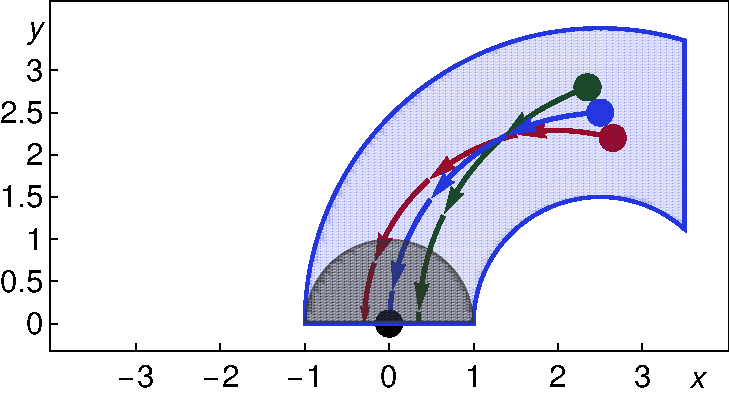
\includegraphics[width=0.3\textwidth]{graphics/fig-ode3.pdf}
\caption{Annular section through the (blue) waypoint $(2.5,2.5)$. Trajectories from the displaced green and red waypoints with slightly different curvatures remain within the annulus.}\label{fig:circlestaging}
\label{fig:circlestaging}
\end{figure}

The \emph{admissibility} test $\ptest{\admiss}$ checks that the chosen $\avar$ will take the robot to its goal with a safe speed limit, by \emph{predicting future motion} of the robot.
We illustrate this with the upper bound conditions.
The bound will be satisfiable after one cycle if either the chosen acceleration $\avar$ already maintains speed limit bounds ($\vvar \leq \vhvar \land \vvar{+}\avar\Tvar \leq \vhvar$) or when there is enough distance left to restore the limits before reaching the goal.
For straight line motion ($\kvar=0$), the required distance can simply be found by integrating acceleration and speed:
\begin{equation*}
\underbrace{\vvar\Tvar+\frac{\avar}{2}\Tvar^2}_{\mathclap{\text{distance in time}~\Tvar}} + \frac{(\overbrace{\vvar{+}\avar\Tvar}^{\mathclap{\text{speed in time}~\Tvar}})^2-\vhvar^2}{2\Bvar} + \veps \leq \lnorm{(\xgvar,\ygvar)}
\end{equation*}
where $\avar \in [-\Bvar,\Avar]$.
The extra factor of $(1 + \abs{k}\veps)^2$ for curved motion accounts for the fact that an arc along the inner side of the annulus is shorter than one along the outside (\rref{fig:circlestaging}).

\subsection{Proofs}
In contrast to prior works~\cite{DBLP:journals/ijrr/MitschGVP17}, this work contains both safety and liveness proofs for the full 2D dynamics.\footnote{In the interest of full disclosure, the modeling and proof sections were largely performed by collaborators in this work. The present author provided simulations, writing, integration with \VeriPhy and advice on the modeling and proof tasks. In contrast, the modeling and proofs in the proposed work are to be performed by the present author}.
In many ways, this lays a foundation for the proposed work because a proof of winnability for a hybrid game will contain both liveness-like (strategy for our player) and safety-like components (strategy for the opponent).
Taken at surface value, the safety theorem says that speed limits are obeyed whenever the robot reaches a waypoint
\begin{theorem}[Safety]
\label{thm:safe}
The following \dL formula is valid:
\begin{align*}
&\Avar{>}0 \land \Bvar{>}0 \land \Tvar{>}0 \land \veps{>}0 \land \linv \limply \\
&\dbox{\prepeat{(\ctrl;\plant)}}{\big(\enorm{(\xgvar,\ygvar)} \leq \veps \limply \vvar \in [\vlvar,\vhvar]\big)}
\end{align*}
\end{theorem}
Taken more broadly, safety also includes the fact that the robot always remains within an $\epsilon$ annulus around the arc leading to the waypoint, which arises as part of the loop invariant used to prove \rref{thm:safe}.
The first four assumptions ($\Avar{>}0 \land \dots \land \veps{>}0$) are basic sign conditions on the symbolic constants used in the model. 
The final assumption, $\linv$, is the loop invariant.
The full definition of $\linv$ is deferred to \rref{sec:robostage}.
We write $\enorm{(\xgvar,\ygvar)}$ for the Euclidean norm $\sqrt{\xgvar^2 + \ygvar^2}$ and consider the robot ``close enough'' to the waypoint when $\enorm{(\xgvar,\ygvar)} \leq \veps$ for our chosen goal size $\veps$.
%The theorem states that no matter which (admissible) control decisions are made, whenever the vehicle is in the goal region of size $\veps$, it obeys the speed limit $\vvar \in [\vlvar,\vhvar]$.
While this captures the desired notion of safety, it does not prove that the robot can actually reach the goal, which is a \emph{liveness} property:
\begin{theorem}[Liveness]
\label{thm:liveness}
The following \dL formula is valid:
\begin{align*}
&\Avar{>}0 \land \Bvar{>}0 \land \Tvar{>}0 \land \veps{>}0 \land \linv \limply \\
&\dbox{\prepeat{(\ctrl;\plant)}}{\Big( \vvar{>}0 \land \yvar{>}0 \limply }\\
&\ \ \ \ \ddiamond{\prepeat{(\ctrlliv;\plant)}}{\big(\enorm{(\xgvar,\ygvar)} \leq \veps~\land~\vvar \in [\vlvar,\vhvar]\big)} \Big)
\end{align*}
%where $\ctrlliv$, as before, controls $\avar$.
\end{theorem}

This theorem has the same assumptions as \rref{thm:safe}. 
It says that no matter how long the robot has been running ($\dbox{\prepeat{(\ctrl;\plant)}}{}$), 
then if some simplifying assumptions still hold ($\vvar{>}0\land\yvar{>}0$) 
the controller can be continually run ($\ddiamond{\prepeat{(\ctrlliv;\plant)}}{}$) with admissible acceleration choices $(\ctrlliv)$ to reach the present goal \((\enorm{(\xgvar,\ygvar)} \leq \veps)\) within the desired speed limits \((\vvar \in [\vlvar,\vhvar])\).
The simplifying assumptions $\vvar{>}0\land\yvar{>}0$ say the robot is still moving forward and the waypoint is still in the upper half-plane, i.e., we have not run \emph{past} the waypoint.

The liveness theorem is invaluable because it validates the \dL model: if it were not even possible at the level of the \dL model to achieve liveness, then it would be absolutely impossible at the level of implementation to achieve liveness.
Because it is undesirable to change the model drastically once implementation has started (i.e., delays in modeling and verification will trickle down to greater delays in implementation and testing), it is valuable to have this confidence in the model before implementation even begins.
Moreover, the combination of safety and liveness gives us confidence that a game generalization of this proof will succeed, as the main components of a game proof are liveness and safety reasoning.

\subsection{Simulations} 
In order to claim that \VeriPhy has been evaluated on a realistic system implementation, it is essential that we choose a simulation platform that is reasonably faithful to the physics of actual autonomous cars.
For this purpose we chose the AirSim~\cite{shah2018airsim} simulator, which is notable for combining top-notch visuals, reasonable physics, and an open-source code base that is particularly friendly to modification.
While some aspects of the underlying physics engine are closed-source, many aspects are open to customization, including for example the details of wheels and suspensions, and the center of gravity.
For this reason and because AirSim has been successfully applied in dozens of projects, we have good reason to believe its physics model is more faithful than any purpose-built one-off simulation would be.

The author implemented several bang-bang and PD (proportional-derivative) controllers in AirSim as well as several environments which provided a variety of driving conditions with turns of different radii.
The environments and the evaluation results are summarized below:
\begin{figure*}[tb]
\centering
\begin{minipage}[b]{2in}\centering
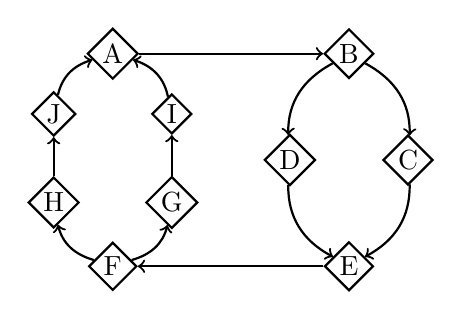
\begin{tikzpicture}[->,draw,thick,yscale=0.9,inner sep=1pt]
\tikzstyle{arc}=[circle,draw]
\tikzstyle{line}=[rectangle,draw]
\tikzstyle{way}=[diamond,draw]
\node[way] (a) at (1,3) {A};
\node[way] (b) at (4,3) {B};
\node[way] (c) at (4.75,1.5) {C};
\node[way] (d) at (3.25,1.5) {D};
\node[way] (e) at (4,0) {E};
\node[way] (f) at (1,0) {F};
\node[way] (g) at (1.75,0.90) {G};
\node[way] (h) at (0.25,0.90) {H};
\node[way] (i) at (1.75,2.15) {I};
\node[way] (j) at (0.25,2.15) {J};
\draw (a) -> (b);
\draw (b) edge [bend left] node {} (c);
\draw (b) edge [bend right] node {} (d);
\draw (c) edge [bend left]node {} (e);
\draw (d) edge [bend right] node {} (e);
\draw (e) -> (f);
\draw (f) edge [bend left]  node {} (h);
\draw (f) edge [bend right] node {} (g);
\draw (h) -> (j);
\draw (g) -> (i);
\draw (j) edge [bend left]  node {} (a);
\draw (i) edge [bend right] node {} (a);
\end{tikzpicture}
\subcaption{Example mission}\label{fig:patrol-mission-plan}\end{minipage}
\begin{minipage}[b]{1.51in}\centering

\includegraphics[width=1.51in,clip,trim=0 0 0 50]{graphics/airsim.png}
\subcaption{Simulator}\label{fig:simulator}\end{minipage}
%\begin{minipage}[b]{.3\linewidth}\centering
%\includegraphics[width=1.95in]{graphics/robot.jpg}
%\subcaption{RC car}\label{fig:rccar}
%\end{minipage}
\begin{minipage}[b]{0.15\textwidth}\centering
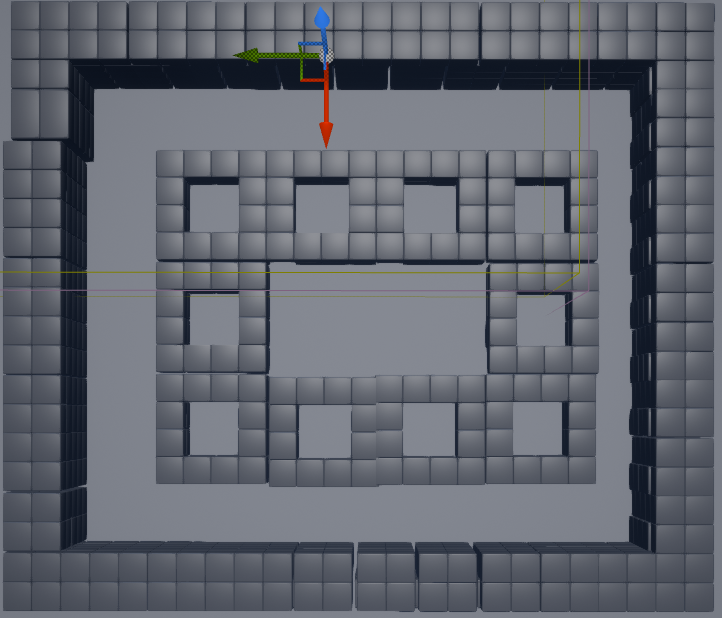
\includegraphics[width=1in]{graphics/screen1.png}
\subcaption{Rectangle}\label{fig:rect}\end{minipage}
\begin{minipage}[b]{0.15\textwidth}\centering
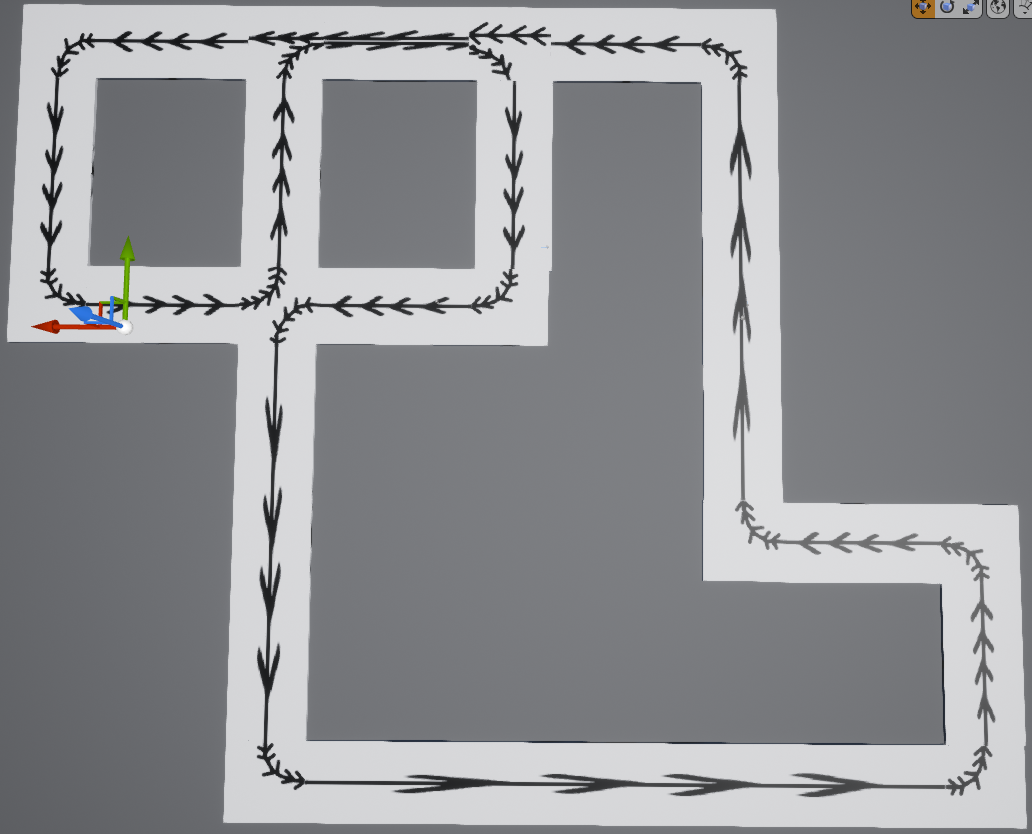
\includegraphics[width=1in]{graphics/screen2.png}
\subcaption{Tight turns}\label{fig:turns}\end{minipage}
\begin{minipage}[b]{0.15\textwidth}\centering
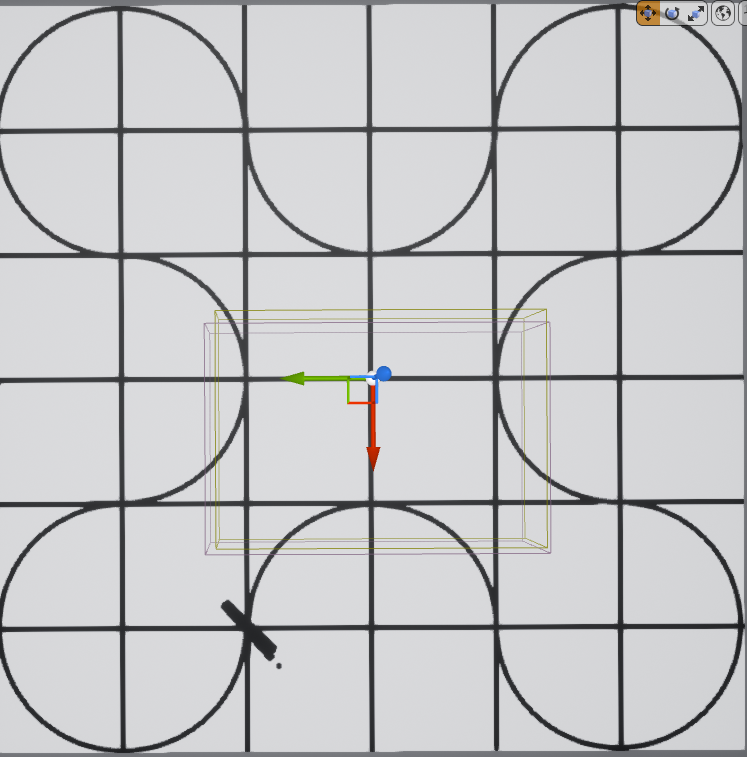
\includegraphics[width=0.8in]{graphics/screen3.png}
\subcaption{Large clover}\label{fig:clover}\end{minipage}
\caption{Implementation and environments built in AirSim}
\label{fig:patrol-plan}
\end{figure*}

\begin{table*}
\caption{Average speed, Monitor failure rates, plant violation rates, for AirSim and human driver in Rectangle, Turns, and Clover for Patrol missions}
\label{tab:results}
\centering
\begin{tabular}{l|l|l|l|l|l|l|l|l|l|l|l|l|l|l|l}
\bottomrule        & \multicolumn{5}{|c|}{Avg.\ Speed (m/s)} & \multicolumn{5}{c|}{Ctrl Fail.} & \multicolumn{5}{c|}{Plant Fail.} \\
World   & BB   & \textbf{PD1}   & PD2   & PD3     & Human     & BB     & \textbf{PD1}      & PD2    & PD3    & Human  & BB    & \textbf{PD1} & PD2   & PD3 & Human \\\toprule
Rect    & 9.2  & \textbf{6.24}   & 8.47 &  13.5   & 12.6      & 1.4\%  & \textbf{0\%}      & 0\%    & 0.17\% & 3.0\%  & 9.8\% & \textbf{1.8\%} & 1.2\%  & 4.0\%   & 10.5\%  \\
Turns   & 8.3  & \textbf{4.54}   & 5.93 &  10.4   & 10.8      & 3.0\%  & \textbf{0\%}      & 3.3\%  & 0.75\% & 3.5\%  & 11\%  & \textbf{0.2\%} & 0.4\%  & 3.1\%   & 5.63\%  \\
Clover  & 13.8 & \textbf{13.9}   & 18.2 &  29.8   & 29.3      & 6.6\%  & \textbf{0.3\%}    & 0\%    & 0.32\% & 0.66\% & 28\%  & \textbf{1.7\%} & 44\%   & 38.1\%  & 24.4\%
\end{tabular}
\end{table*}
\rref{tab:results} gives the results of several controllers (PD1 is the slowest PD controller, PD3 the fastest) as well as a human pilot (the author) on all environments.
Overall, the slow PD controller had the best monitor failure rates of any controller.
Qualitatively, the results tell us that while perfect failure 0\% rates are not always attainable, low failure rates are achievable in practice, where low control failure rates mean that the fallback controller will rarely need to engage and low plant failure rates mean that because physical assumptions are rarely violated, the formal guarantees provided by \VeriPhy are applicable almost all the time.

Aside from the concrete numbers provided by the simulations, perhaps the most important conclusion is that such a simulation could be developed and monitored in the first place.
Throughout the development of this section, many iterations of the models, proofs, and simulations were developed: in order to make the proofs feasible, the models would be simplified, then when monitor failures were detected, the models would be relaxed to improve the failure rate.
Low failure rates not only speak to the success of the implementation, but they say even more about the success of the model: any time the model were too restrictive to account for the values given by the AirSim sensors and controllers, the monitor would have failed.
The fact that they fail rarely attests that the model can account for the control decisions and physical dynamics that arise in practice.
Because it was not until this chapter that a completely formal link between \dL and CPS execution had been developed, this itself was long a point of curiosity.

\subsection{Related Work}
Related work in formal methods and robotics has applied synthesis and verification to safe control of robotic systems.
The present work is unique among these in its use of a verified-safe sandbox controller to enforce compliance between the implementation and formal model for a realistic robot simulation with an expressive correctness guarantee.

\subsubsection{Synthesis for Planning and Control}
A significant focus of related work is the synthesis of motion plans from high-level specifications.
These works can be fruitfully combined with ours, providing a high-level plan to be followed, but none of them address correctness of low-level controllers that implement the plan, and all trust the correctness of their kinematic models:
\begin{itemize}
\item The tools LTLMoP~\cite{DBLP:conf/iros/FinucaneJK10} and TuLiP~\cite{DBLP:conf/IEEEcca/FilippidisDLOM16} can synthesize robot controls that satisfy a high-level temporal logic specification.
However, they depend on accuracy of their kinematic models, which assume  discrete-space and discrete-time, and the guarantees are not end-to-end.
\item Bisimulation~\cite{871304} is used to synthesize plans based on hybrid dynamics~\cite{DBLP:conf/cdc/BhatiaKV10,DBLP:journals/automatica/FainekosGKP09}, but assumes model compliance and cannot ensure low-level controller correctness.
\item Controllers have been synthesized:
\begin{inparaenum}[\it i)]
\item from temporal logic specifications for linear systems~\cite{DBLP:journals/tac/KloetzerB08},
\item for adaptive cruise control~\cite{DBLP:journals/tcst/NilssonHBCAGOPT16}, tested in simulation and on hardware, and
\item from safety proofs~\cite{DBLP:conf/emsoft/TalyT10} for switched systems using templates,
\end{inparaenum}
but those works assume model compliance and cannot ensure low-level controller correctness.
\end{itemize}

\subsubsection{Offline Verification for Planning and Control}
In contrast to online synthesis of a correct plan and/or controller, offline verification shows correctness before the fact, which is often more tractable and eases incorporation of custom controllers.
Much of the verification in robotics focuses on hybrid systems models;
common approaches are reachability analysis~\cite{DBLP:conf/cav/FrehseGDCRLRGDM11} and theorem proving~\cite{DBLP:conf/cade/FultonMQVP15}.
\begin{itemize}
\item 1D straight-line motion was addressed both in \dL (for direct velocity control)~\cite{DBLP:conf/pldi/BohrerTMMP18} and with reachability analysis~\cite{chen2015benchmark},
 but the 2D motion demanded by real robots introduces novel modeling, verification, and implementation challenges: our invariants and controllers must account for curved motion, acceleration, and uncertain sensing and actuation.
\item
 Unbounded-time 2D obstacle avoidance and 1D liveness have also been proved in \dL~\cite{DBLP:conf/rss/MitschGP13,DBLP:journals/ijrr/MitschGVP17}.
A paper proof of liveness using \dL rules assumed perfect sensing and constant speed \cite{DBLP:journals/corr/abs-1709-02561}.
 Their controllers, like ours, are closely related to the classic Dynamic-Window~\cite{DBLP:journals/ram/FoxBT97} control algorithm.
 In contrast to the prior \dL effort, we offer stronger results, including 2D liveness, waypoint-following, and end-to-end correctness.
\item
  A planner for ground vehicles was verified~\cite{DBLP:conf/atva/RizaldiISA18} in Isabelle/HOL.
  Unlike our work, it does not address low-level control and implementation correctness.%, but could be used to provide an input plan.
\end{itemize}
%  We provide a simpler model which enabled LEEV of our implementations with \VeriPhy, whereas the model of~\cite{DBLP:journals/ijrr/MitschGVP17} is too restrictive (i.e., the synthesized monitor would always fail in practice).
%\item Reachability is most-often used in design, but can also be used for model-predictive control~\cite{Bemporad2000PerformanceDR}.
%Hybrid systems theorem-proving in \dL~\cite{DBLP:books/sp/Platzer18} with \KeYmaeraX~\cite{DBLP:conf/cade/FultonMQVP15} is typically less automated, with unique advantages in system complexity (polynomial ODEs), property complexity (unbounded-time safety and liveness), and rigor (small\cite{DBLP:conf/cade/FultonMQVP15}, verified~\cite{DBLP:conf/cpp/BohrerRVVP17} trusted base).  Control strategies for ground vehicles are well-studied.
%Reachability for liveness has been investigated~\cite{BEMPORAD2001382}.

\subsubsection{Online Verification}
In contrast to offline verification, online (or runtime) verification uses runtime checks to enforce safe operation.
\begin{itemize}
\item The basis of online verification is the SIMPLEX~\cite{Krogh1998TheSA} method, which uses a trusted monitor to decide between an untrusted controller and trusted fallback.
\item The \VeriPhy~\cite{DBLP:conf/pldi/BohrerTMMP18} toolchain for \dL, which we use, extends SIMPLEX by ensuring the monitor is correct-by-construction, formally proving the safety of the resulting system, and automatically maintaining safety down to machine code implementation.
High-Assurance SPIRAL~\cite{DBLP:journals/csm/FranchettiLMMGPPKMFJPV17} is another implementation toolchain for \dL, but does not provide formal end-to-end guarantees, and neither has been used to develop an end-to-end system capable of free-range 2D driving until now.
\item Runtime reachability analysis has been used for car control~\cite{DBLP:journals/trob/AlthoffD14}, but relies on correctness of the model and of the analysis implementation.
Since reachability tools rely on large, complicated codebases and models are challenging to get right, these assumptions present a correctness gap which stands in the way of an end-to-end argument.
\end{itemize}

\subsubsection{Simulation}
Simulation is an essential part of evaluating models and designs for any robotic system.
Multiple simulation platforms are available, of which AirSim~\cite{shah2018airsim} is a recent platform for UAVs and autonomous cars.
Other simulators would likely have worked as well, but we chose AirSim because it is configured with high-fidelity physical and visual models out of the box, reducing the chances of introducing modeling errors.

In short, while verification of robotics is well-studied, few works have addressed end-to-end guarantees with the highest level of rigor, and in this paper we develop the first realistic, end-to-end system with an expressive correctness guarantee of safety and liveness for 2D waypoint following.

\chapter{Proposed Work: \CdGL: Constructive Differential Game Logic}
\label{ch:cdgl}
Throughout this thesis, end-to-end verification is conceived as the problem of placing the correctness of realistic CPS on the most rigorous, formal logical foundation possible.
The logic we use to verify a CPS model (thus far, \dL) is then the centerpiece and our understanding of its foundations are of central importance.
In \rref{ch:logical-foundations}, we started at the centerpiece and dug inward: we established a more rigorous foundation for \dL as it is used in practice in the theorem prover by building a formally verified prover core and by providing a unified foundation for the grabbag of features that arise in practice.
In \rref{ch:end-to-end-v}, we started at the centerpiece and dug outward: model-driven monitor synthesis connects CPS implementations to their formal models;
we showed that this connection can be made with full rigor for serious models and their implementations, placing our understanding of implementation-level safety on firm footing.

In the proposed work, the time has come to question the centerpiece itself.
Vanilla \dL has been used thus far in part because it comes with rich theoretical backing, a mature implementation, and prior cases studies for inspiration and comparison.
However, as a logic, it hardly exists in isolation: A family of logics including \QdL, \SdL, and \dGL have explored the addition of distributed, stochastic, and adversarial dynamics to hybrid systems, respectively.
Further unexplored logical questions await: notably, all of the above logics are classical.
When constructive logic is a key tool in software verification, we must earnestly ask what could be gained for end-to-end CPS verification by adopting constructive foundations.
We must also ask which member of the \dL family (which might not even be discovered yet) is best suited for end-to-end CPS verification.

This thesis views end-to-end verification as resolving the concerns of three entities:
the logician concerned with rigorous foundations, the practitioner concerned with software artifacts resulting from verification, and the logic-user, concerned primarily with simplicity and readability of their models and the ease of their proofs.
We have already satisfied the logician: we have made \dL proofs in \KeYmaeraX indisputable.
However, we argue that constructivity and games both have crucial advantages for the practitioner and logic-user.
Thus, a constructive games logic (\CdGL) is the optimal foundation to resolve the concerns of all three.

The completed sections of the thesis have revealed several weaknesses from the practitioner's perspective:
\begin{itemize}
\item
The state-of-the-art supports only synthesis of control and plant monitors, not controllers nor plant simulations.
The programmer might be content to write the controller themselves, but they are less content to prove for themselves that it always satisfies the monitor.
For the programmer, the CPS has not been proven correct unless they know the monitor will be satisifed!
Plant simulations are also valuable because they provide a complementary way to evaluate and understand a model, which is more familiar to most programmers.
\item
The state-of-the-art in synthesis lacks robustness, often restricting the user to special cases and failing to synthesize otherwise.
Important control paradigms such as model-predictive control do not fall within the supported special cases, nor do any controllers containing loops.
The \ModelPlex synthesis approach started from the assumption that the model alone is sufficient, which was then falsified by the need to handle complex models, especially those whose plants are not nilpotent.
The resulting approach scrapes invariant information from proofs in an ad-hoc fashion to aid synthesis.
While the invariant information is essential, the ad-hoc nature stands in the way of robustness.
\item
The synthesized monitors are not tight.
The arithmetic approximations used in \rref{sec:veriphy} are conservative, and in practice can be prohibitively so, to the extent that significant cleverness is exerted in tweaking units of measure to avoid overflow errors.
The implementation of arithmetic in synthesis is a fundamental question, but the present answer of integer interval arithmetic demands too much of the programmer.
\end{itemize}
All these concerns are addressed by the combination of games and constructivity:
\begin{itemize}
\item
The main challenge in synthesizing a controller is deciding which control path to take (for example, acceleration vs. braking) when multiple options are plausible.
All such decisions are captured by a proof of the shape $\ddiamond{\ctrl}{\phi}$: in proving a diamond property, we have specified which path to take in order to achieve $\phi$.
Such synthesis is only possible in general when the proof is constructive: the state-of-the-art proof technique for such properties in fact applies the law of excluded middle to undecidable propositions, so constructivity is anything but a theoretical concern.
In this chapter, we will incorporate an alternative proof method only case-analyzes decidable properties so that synthesis is possible.
Games also play a part in controller synthesis: A typical game proof supports a diamond proof for control and a box proof for plant, making it simple to synthesize both a controller and monitor together.
\item
Robustness issues in the state-of-the-art are simply a side effect of the fact that there is no proof representation available that closely corresponds to intuitive notions of control and monitoring.
While proof representations are available, including one developed by the author, these representations use a low-level classical Hilbert calculus with no obvious computational interpretation and no obvious correspondence to intuitive ``human-level'' proofs.
Developing a proof-theoretic semantics with a computational interpretation of proof terms is par for the course in constructive logic.
By developing such semantics for \CdGL, we will lay the foundation for robust implementation of proof-driven synthesis.
\item
Conservativity is a consequence of the chosen arithmetic implementation: fixed-precision interval arithmetic.
Better libraries might alleviate the practical concern, but constructive mathematics provides a more general answer: computable reals.
Constructive proofs in \CdGL have the convenient property that whenever a proof of $\ddiamond{\ctrl}{\phi}$ exists, a controller exists which uses only \emph{total} computations on computable reals (e.g.\ the controller will never attempt to compare two reals for exact equality).
Certainly interval arithmetic has its own advantages in performance, but with computable reals we resolve conservativity issues conclusively.
\end{itemize}

For the logic-user:
\begin{itemize}
\item
Short, simple models are desirable.
Longer models are more likely to contain mistakes, and modeling mistakes are the hardest kind to catch as we cannot simply ``prove'' their presence or absence.
As \rref{sec:planar-driving-system} and \rref{ex:driving-system} show, hybrid systems models are typically much more complicated than their hybrid game counterpart, because strategic choices must be modeled in the hybrid system which in games are deferred to the proof.
Thus, games generally (\dGL or \CdGL) eliminate a prominent source of needless model complexity.
\item
Beyond reducing complexity, games models preclude common mistakes which have led even experienced researchers to write vacuous models in practice.
Specifically, in a standard \dL safety proof, safety is proven only for states from which at least one guard of the controller is satisfied.
An intuitive notion of safety requires that at least one guard is satisifed in each state (the controller is \emph{total}), which is often false when models are not written carefully.
In games, we can (and by default do) require that controllers satisfy \emph{co-safety}, which implies any faulty, non-total controller will be caught when at proof time since a co-safety proof will necessarily fail.
Catching such mistakes is important because otherwise the logic-user, having proved a vacuous theorem, would assume their system is safe when in fact \emph{nothing} of note has been proven.
\item
For many programmers, formal proofs are more intimidating than code and thus possess a steeper learning curve.
While not a focus of the present thesis, a computational interpretation opens up the possibility of writing \CdGL proofs by writing the code that implements a winning strategy.
We suggest that such an approach would ease adoption of proofs for CPS.
\end{itemize}

Lastly, even though the logician's foundational concerns have been adequately addressed in the previous chapters, there are independent motivations for \CdGL from a foundational, theoretical perspective:
\begin{itemize}
\item As discussed in related work, constructive program logics are a nearly-unexplored topic, and even constructive modal logic generally is a lightly explored field.
\CdGL is not only a generalization of  \dGL and \dL, but also of (Harel's) First-order Dynamic Logic and (Parikh's) Game Logic, which itself generalizes (von Pratt's) PDL and (Peleg's) Concurrent Dynamic Logic.
In developing \CdGL, we indirectly develop the first serious constructive treatment for all the above logics as well, specifically the first to feature a full proof-theoretic treatment based on proof terms and their normalization.
It is also the first treatment of any of the above to support standard constructive properties such as the Existential Property
\item
The Curry-Howard correspondence, wherein propositions are interpreted types and proofs are interpreted as programs,
has for many years been the backbone of cross-pollination between programming languages and logic research.
\CdGL gives the first understanding of Curry-Howard for game logics or any dynamic logic:
Proofs of $\ddiamond{\alpha}{\phi}$ and $\dbox{\alpha}{\phi}$ are understood computationally as winning strategies, for the P-player and N-player, respectively.
In the special case, they are understood as \emph{controlling} program $\alpha$ to achieve $\phi$ or \emph{monitoring} an execution for compliance with $\alpha,$ which ensures $\phi$ as postcondition.
This substantiates the claim that such proofs suffice for synthesis, and we posit that this correspondence is applicable to \emph{any} nondeterministic program logic.
\footnote{One could also apply this interpretation to deterministic logics, but they lack our motivations of synthesis and monitoring, which is perhaps the reason this interpretation never developed sooner}
\end{itemize}


%\textrm_{\alpha{Sys}}

\section{Related Work}
\newcommand{\semiset}[2]{\{#1~|~#2\}}
\section{Syntax}
The term language of \CdGL is that of \dL:
\[\theta \bebecomes  q \alternative x \alternative \theta + \eta \alternative \theta \cdot \theta \alternative \der{\theta}\]
where $q \in \mathbb{Q}$ is a literal, $x$ a variable, $\theta + \eta$ a sum, $\theta \cdot \eta$ a product and $\der{\theta}$ a derivative.

The formulas of \CdGL are:
\[\phi \bebecomes \theta > \eta \alternative  \phi \land \psi \alternative \phi \lor \psi \alternative \phi \limply \psi \alternative \bot \alternative \ddiamond{\alpha}{\phi} \alternative \dbox{\alpha}{\phi} \alternative \forall{x}{\phi} \alternative \exists{x}{\phi}\]
where $\theta > \eta$ is true when $\theta$ is greater than $\eta,$ $\phi \land \psi$ is true when $\phi$ and $\psi$ are both true, $\phi \lor \psi$ is true when either $\phi$ or $\psi$ is true (and we know which one), $\phi \limply \psi$ is true when $\psi$ is true under the assumption that $\phi$ is true, and $\bot$ is not true.
$\ddiamond{\alpha}{\phi}$ is true when Angel has a strategy for $\alpha$ to reach the region where $\phi$ is true (and we know which strategy, and we know why $\phi$ is true in the end).
Likewise, $\dbox{\alpha}{\phi}$ is true when Demon has a strategy for $\alpha$ to reach the region where $\phi$ is true.
$\lforall{x}{\phi}$ is true when $\phi$ is true under the assumption that $x$ is a fresh (real-valued) variable.
Likewise, $\lexists{x}{\phi}$ is true when $\phi$ is true under some assignment of $x$ (and we know which one).

Since \CdGL is a constructive logic, classical duality axioms such as $\phi \lor \psi \equiv \neg(\neg \phi \land \neg psi)$ do not hold, and thus none of the above constructs are derived.
Even in a constructive logic, however, the constructs $\neg \phi \equiv (\phi \limply \bot), \phi \lequiv \psi \equiv (\phi \limply \psi \land \psi \limply \phi),$ and $\theta \geq \eta \equiv \neg(\eta > \theta)$ are derived.
The equivalence $\theta \geq \eta \equiv \neg(\eta > \theta)$ is standard in constructive analysis, but nonstrict inequalities will merit special attention since equality on reals is undecidable, and thus nonstrict inequalities are as well.
For example, the trichotomy axiom of classical analysis:
\[\theta < \eta \lor \theta = \eta \lor \theta > \eta\]
is false constructively, as it is undecidable which of three cases holds.

In \CdGL, hybrid games follow the same syntax as in \dGL, except that all formulas appearing in games are \CdGL formulas.

\section{Example System}
As a case study for \CdGL, we propose reproducing the 2D planar robot of \rref{sec:ground-robotics} as a hybrid game, and providing a constructive proof that the robot can reach its waypoints while maintaining its speed limits.
In order to assess the feasibility of this task early, without access to an implementation of \CdGL, we propose performing the proof in classical \dGL in \KeYmaeraX and inspecting by hand that the proof uses only constructive reasoning.
We give the hybrid game model here.
The plant is identical to that of \rref{sec:ground-robotics}: the robot is fixed at the origin facing toward the +y axis, while the waypoint moves relative to it:
\begin{align*}
\plant\equiv \{&\D{\xgvar}=-\vvar~\kvar~\ygvar,~\D{\ygvar}=\vvar~(\kvar~\xgvar-1),~\D{\vvar}=\avar,~\D{\tvar}=1 \\
 &\&~\tvar\leq \Tvar ~\land~ \vvar \geq 0\} %  ~\land~ yg > 0
\end{align*}
The conditions $\annul$ and $\planreq,$ which say the waypoint and robot are on the specified annulus, and that the waypoint is achievable, respectively, are also as before:
{\small\begin{align*}
\annul &~\mequiv~\abs{\kvar}\veps \leq 1 \land \Big|\frac{ \kvar~\left(\xgvar^2 +\ygvar^2 - \veps^2 \right)}{2} - \xgvar\Big| < \veps\\
%ygvar>0 included for consistency with the proof (it is also monitored to satisfy our liveness assumption)
\label{eq:planReq} \planreq &~\equiv \annul \land \ygvar{>}0 \land 0{\leq}\vlvar{<}\vhvar \land \Avar\Tvar{\leq}\vhvar-\vlvar \land \Bvar\Tvar{\leq}\vhvar-\vlvar
\end{align*}}

The main change is in the controller.
In the systems setting, the controller needed to express a condition $\admiss$ which specified the allowable accelerations in each case.
In the games setting, the acceleration is existentially quantified in the model, and choices of acceleration are merely part of the proof:
{\small
\[\ctrl~\equiv~ \pdual{(\prandom{(\xgvar,\ygvar)};\,\prandom{[\vlvar,\vhvar]};\,\prandom{\kvar};\,\ptest{\planreq})};\,\prandom{\avar}\]
}

We propose to prove a winnability theorem saying the robot can always control its way to the goal region within its speed limits.
\begin{theorem}[Angel Winnability]
\label{thm:angel-wins}
The following \dL formula is valid:
\begin{align*}
&\Avar{>}0 \land \Bvar{>}0 \land \Tvar{>}0 \land \veps{>}0 \land \linv \limply \\
&\ddiamond{\prepeat{(\ctrl;\pdual{\plant})}}{\big(\enorm{(\xgvar,\ygvar)} \leq \veps \land \vvar \in [\vlvar,\vhvar]\big)}
\end{align*}
where $J$ is the loop invariant as defined in \rref{sec:ground-robotics}.
\end{theorem}
In this form, \rref{thm:angel-wins} corresponds to the liveness, \rref{thm:liveness}.
However, we propose also to generalize \rref{thm:angel-wins} slightly, thus proving \rref{thm:liveness} and \rref{thm:safe} (safety) in one go.
\begin{theorem}[Generalized Angel Winnability]
\label{thm:angel-wins-gen}
The following \dL formula is valid:
\begin{align*}
&\Avar{>}0 \land \Bvar{>}0 \land \Tvar{>}0 \land \veps{>}0 \land \linv \limply \\
&\ddiamond{\prepeat{(\ctrl;\pdual{\plant};\ptest{J})}}{\big(\enorm{(\xgvar,\ygvar)} \leq \veps \land \vvar \in [\vlvar,\vhvar]\big)}
\end{align*}
where $J$ is the loop invariant as defined in \rref{sec:ground-robotics}.
\end{theorem}
That is, after Demon chooses the duration of the plant, Angel must prove that the loop invariant $J$ still holds.
Recall that the invariant $J$ includes as conjuncts the facts that the robot is on the annulus and has sufficient distance remaining to achieve its speed limit.
To win the generalized game, Angel must be able to prove that it is on track to the waypoint (both in position and velocity) at \emph{whatever} point Demon chooses, thus at every one of the uncountably many points in time.
This is exactly what safety ought to constitute.
Because we simply added a test to the previous model, whenever Angel wins the modified game they have still achieved liveness.
It is simply harder now, as they must never violate safety in the process of achieving liveness.

The example demonstrates several advantages of hybrid games proving generally over hybrid systems.
Not only is the model shorter, waypoint-following exhibits turn-taking behavior which is challenging to characterize in a hybrid system.
The Angel player must follow an arbitrary waypoint, i.e., one chosen by Demon.
In order to make victory for Angel even possible, the responsibility is Demon's to choose a waypoint that is feasible.
Expressing this turn-taking in \rref{thm:live} is cumbersome, while in \rref{thm:angel-wins-gen}, it falls naturally out of the fact that acceleration is controlled by Angel while all else is up to Demon.
Lastly, we have the advantage that safety and liveness need not be proved separately, but can be combined as a single winnability theorem.
This obviously saves time and energy, but there is a conceptual advantage as well: in the systems setting, we must prove \emph{all} options are safe and that \emph{one} is live.
In the games setting, we can simply prove that \emph{one} strategy is safe-and-live, so for states our strategy will never enter, we need not even consider safety.

The winnability approach ought to apply to any \emph{reach-avoid} problem for a control-plant loop, i.e., any theorem of form:
\[\text{pre} \limply \ddiamond{\prepeat{(\ctrl;~\pdual{(\plant)};~\ptest{\text{safe}})}}{\text{live}}\]
Within the hybrid systems literature, and certainly within the \dL literature, most systems can be expressed as control-plant loops, and the most important properties are reach-avoid properties or special cases thereof.
Thus we are justified to claim that a wide array of verification tasks would benefit from the simplicity provided by modeling and proving with games.

\section{Semantics}
Several styles of semantics are widely used for constructive logics, and each has its own advantages.
We present several semantics here, since the remaining tasks (proof term semantics, theoretical results) will inform the choice between them.
\newcommand{\allcon}{\allregion}
\newcommand{\somesemi}[2]{\epsilon #1~|~#2}

\subsection{Intuitionistic Kripke Semantics with Computability}
Kripke semantics can be generalized to the intuitionistic setting.
In intuitionistic Kripke semantics, the world is typically understood epistemically, i.e., the semantics are not parameterized over the world as it is, simply what is known about the world.
We can then understand an epistemic state as a region $Y \subseteq \allstate$ over \emph{actual} states: to know $Y$ is to know that we are in one of the states $\omega \in Y$.
Thus to know $\allstate$ is to know nothing and to know $\emptyset$ is to know a contradiction (has been reached). 

Given this understanding, we reach a semantics with much a similar flavor to the classical Kripke semantics.
The formula semantics $\fint{\phi}{}$ is no longer read as the region on which $\phi$ is true, but the the (unique) largest region from which Angel has a strategy to prove $\phi$.
\newcommand{\mto}{\rightharpoonup}
\begin{align*}
  \fint{\theta > \eta}{}         &= \{\om~|~\tint{\theta}{\om} > \tint{\eta}{\om}\}\\
  \fint{\phi \land \psi}{}       &= \fint{\phi}{} \cap \fint{\psi}{}\\
  \fint{\phi \lor \psi}{}        &= \bigcup\{A \cup B \subseteq \allstate~|~\exists f:\allstate\mto 2, f(\om)=0, f(\nu)=1, \om\in A, \nu \in B, A \subseteq \fint{\phi}{}, B \subseteq\fint{\psi}{}\}\\
  \fint{\phi \limply \psi}{}     &= \bigcup\{Z \subseteq \allstate ~|~ Z\subseteq\fint{\phi}{}\text{ implies }Z\subseteq\fint{\psi}{}\}\\
  \fint{\forall{x}{\phi}}{}      &= \{\om~|~\subst[\om]{x}{r}\in\fint{\phi}{}, \text{ all }r\in\reals\}\\
  \fint{\exists{x}{\phi}}{}      &= \{\om~|~\subst[\om]{x}{f(\om)}\in\fint{\phi},\text{ some }f:\allstate\mto \reals\}\\
  \fint{\bot}{}                  &= \emptyset  \\
  \fint{\ddiamond{\alpha}{\phi}} &= \strategyfor[\alpha]{\fint{\phi}{}}\\
  \fint{\dbox{\alpha}{\phi}}     &= \dstrategyfor[\alpha]{\fint{\phi}{}}
\end{align*}
Where $A \mto B$ is the set of computable multi-valued functions from A to B.
We use multi-valued functions rather than typical single-valued functions since they better capture the reasoning which is possible with computable reals:
\begin{inparaenum}
\item The approximate splitting principle used for case analysis on reals will need multivalued functions for most proofs.
\item Multivalued functions support nondeterminism in strategies that single-valued functions do not.
This is useful for example if we ever wish to synthesize a randomized implementation.
\end{inparaenum}

For each construct that requires a choice, the semantics expect the existence of a computable function that resolves the choice.
Most often, intuitionistsic Kripke logics do not explicitly require the existence of such a computable function (but, as a metatheorem, they often exist).
This is a legitimate choice in our case as well, but it would have the symptom that any proof calculus and any proof-theoretic semantics would be incomplete with respect to the intuitionistic semantics.
We can also phrase the choice in philosophical terms: should a strategy which uses classical reasoning be consider a strategy at all?
Should a game even be considered winnable when it is only won with a classical strategy?


%, while $A \to B$ is the set of all computable functions from A to B, and where term semantics are as before.
%In both cases we treat the output as a scalar (i.e. we just assume the interpretation of the multi-valued function is not unique).
%Because even constructive set theories support a collection axiom that converts a multi-valued function to proper function, they can be used more-or-less interchangeably.


The game semantics are given by:
\begin{align*}
  \strategyfor[\ptest{\phi}]{X}      &= \fint{\phi}{} \cup X\\
  \strategyfor[\humod{x}{\theta}]{X} &= \{\om~|~\subst[\om]{x}{\tint{\theta}{\om}} \in X\}\\
  \strategyfor[\prandom{x}]{X}       &= \{\om~|~\subst[\om]{x}{f(\om)} \in X, \text{ some }f:\allstate\mto\reals\}\\
  \strategyfor[\alpha;~\beta]{X}     &= \strategyfor[\alpha]{\strategyfor[\beta]{X}}\\
  \strategyfor[\alpha\cup\beta]{X}   &= \bigcup\{A \cup B \subseteq \allstate~|~\exists f:\allstate\mto 2, f(\om)=0,f(\nu)=1,\om\in A, \nu \in B, A \subseteq\strategyfor[\alpha]{X}, B \subseteq\strategyfor[\beta]{X}\}\\
  \strategyfor[\pdual{\alpha}]{X}    &= \dstrategyfor[\alpha]{X}\\
  \strategyfor[\prepeat{\alpha}]{X}  &= \bigcap\{Z\subseteq\allstate~|~X\cup\strategyfor[\alpha]{Z} \subseteq Z\}\\
  \dstrategyfor[\ptest{\phi}]{X}      &= \fint{\phi}{}^C \cup X\\
  \dstrategyfor[\humod{x}{\theta}]{X} &= \{\om~|~\subst[\om]{x}{\tint{\theta}{\om}} \in X\}\\
  \dstrategyfor[\prandom{x}]{X}       &= \{\om~|~\subst[\om]{x}{r} \in X, \text{ all }r:\reals\}\\
  \dstrategyfor[\alpha;~\beta]{X}     &= \dstrategyfor[\alpha]{\dstrategyfor[\beta]{X}}\\
  \dstrategyfor[\alpha\cup\beta]{X}   &= \dstrategyfor[\alpha]{X} \cap \dstrategyfor[\beta]{X}\\
  \dstrategyfor[\pdual{\alpha}]{X}    &= \strategyfor[\alpha]{X}\\
  \dstrategyfor[\prepeat{\alpha}]{X}  &= \bigcup\{Z\subseteq\allstate~|~Z\subseteq X\cap \dstrategyfor[\alpha]{Z}\}
\end{align*}
It is unclear what semantics would serve us best in the cases $\strategyfor[\prepeat{\alpha}]{X}$ and $\dstrategyfor[\prepeat{\alpha}]{X}$: while fixpoint constructions are widely used in constructive mathematics, fixpoint semantics do not make the termination conditions for a loop explicit.
They might even admit the existence of loops which require undecidable termination conditions.

\subsection{Real Constructive Games, Realizability}
\newcommand{\rzF}[2]{#1 \vdash #2}
\newcommand{\rzA}[3]{\langle{#2}\rangle(#1)=(#3)}
\newcommand{\rzD}[3]{[{#2}](#1)=(#3)}
\newcommand{\rzFst}[1]{#1_0}
\newcommand{\rzSnd}[1]{#1_1}
\newcommand{\rzThd}[1]{#1_2}
\newcommand{\rzFrt}[1]{#1_3}
\newcommand{\rzApp}[2]{#1#2}
\newcommand{\sa}{\omega}
\renewcommand{\sb}{\nu}
\newcommand{\Sc}{\mu}
\renewcommand{\aa}{a}
\newcommand{\ab}{A}
\newcommand{\ac}{\aleph}
\newcommand{\da}{d}
\newcommand{\db}{D}
\newcommand{\dc}{\delta}
\newcommand{\allRz}{\mathcal{R}\mathbf{z}}
Of the possible semantics, Kripke semantics are abstract: truth of a formula implies the existence of a winning strategy, but the strategy does not appear explicitly in the semantics.
Realizability semantics targets a lower level of abstraction: the semantics is parameterized by computable \emph{realizer} functions which implement strategies for Angel and Demon, respectively.
Because realizer semantics are low level, they are less desirable as our fundamental definition of truth, but could be a useful middle step between a completely concrete proof-theoretic semantics and an abstract Kripke semantics.
The realizability semantics consists of three main judgments:
Realizability of a formula $\rzF{\sa,\aa,\da}{\phi}$ holds when the formula $\phi$ is realized by the Angel strategy $\aa$ and Demon strategy $\da$ when starting from state $\sa$.
The Angel realizability judgement $\rzA{\sa,\aa,\da}{\alpha}{\sb,\ab,\db}$ says that after running $\alpha$ from initial state $\sa$ under control of Angel strategy $\aa$ and Demon strategy $\da,$ we will reach state $\sb$ with realizers $\ab$ and $\db$.
The counterpart for Demon is written $\rzD{\sa,\aa,\da}{\alpha}{\sb,\ab,\db}$.
Note that both judgements are written in functional syntax and can be thought of as (partial) functions, because $\sb,\ab,\db$ are always unique.
While hybrid games are themselves highly nondeterministic, the realizers resolve all nondeterminism.

We write $\allRz$ for the set of all realizers.
Per standard practice, realizers are coinductively defined and are untyped, and we do not specify a concrete internal representation.
When a realizer $\aa$ is a coinductive pair, we write $\rzFst{\aa}$ for its first component and $\rzSnd{\aa}$ for its second component.
When a realizer $\aa$ is a function (specifically $A \to \allRz$ for some base type $A$), we write $\rzApp{\aa}{x}$ for the component assigned to some $x:A$.
We implicitly assume throughout that realizers have the right ``type'' (pair or function) for the given program.
To be totally rigorous we should show that realizers are type-correct when extracting realizers from proofs.

The set of realizers $\allRz$ is defined coinductively as the greatest set such that for all $\aa \in \allRz$, at least one of the following holds:
\begin{itemize}
\item $\rzFst{\aa} \in \mathbb{B}$ and $\rzSnd{\aa} \in \allRz$
\item $\rzFst{\aa} \in \mathbb{R}$ and $\rzSnd{\aa} \in \allRz$
\item $\rzFst{\aa} \in \allstate$ and $\rzSnd{\aa} \in \allRz$
\item $\rzApp{\aa}{r} \in \allRz$ for all $r \in \mathbb{B}$
\item $\rzApp{\aa}{r} \in \allRz$ for all $r \in \mathbb{R}$
\item $\rzApp{\aa}{\ab} \in \allRz$ for all $\ab \in \allRz$ (i.e., the set of realizers is super-exponential)
\item $\rzFst{\aa} \in \mathbb{R}$, $\rzApp{\rzSnd{\aa}}{s} \in \allstate$ and $\rzApp{\rzThd{\aa}}{s} \in \allRz$ for all $s \in [0,\rzFst{\aa}]$ and $\rzFrt{\aa}\in\allRz$
\item $\aa = \epsilon$ (the unit realizer, realizes nothing)
\end{itemize}
Because this set is coinductively defined, it includes infinite strategies for infinite plays.
There are several possible treatments of inifinite plays and strategies.
The two simplest treatements, both of which result in the ``finite plays only'' treatment from classical \dGL, are:
\begin{itemize}
\item 
 Interpret the judgements $\rzA{\sa,\aa,\da}{\alpha}{\sb,\ab,\db}$ and $\rzD{\sa,\aa,\da}{\alpha}{\sb,\ab,\db}$ inductively.
 Then they will only ever hold when applied to finite strategies anyway.
\item Quantify over finite traces only in the definition of validity
\end{itemize}
It is a bad idea to allow infinite strategies (with a coinductive interpretation of $\rzA{\sa,\aa,\da}{\alpha}{\sb,\ab,\db}$ and $\rzD{\sa,\aa,\da}{\alpha}{\sb,\ab,\db}$) for either player, 
because they would have a strategy to win every repetition game (for every postcondition, even false) by repeating forever, which is not very helpful.
On some level, it seems more natural to allow infinite plays in boxes than in diamonds, which might simplify metalogical arguments that \CdGL is really talking about CPSs that run forever, but even this would require a careful rethinking of the semantics.

We define the realization judgments recursively:
\begin{align*}
\rzF{\sa,\aa,\da}{\phi \land \psi}        &\text{ iff }\rzF{\sa,\aa 0,\da 0}{\phi}\text{ and }\rzF{\sa,\aa 1,\da 1}{\psi}\\
\rzF{\sa,\aa,\da}{\phi \lor \psi}         &\text{ iff }\rzFst{\aa}=0\text{ and }\rzF{\sa,\rzSnd{\aa},\da 0}{\phi}\\
                                          &\text{ or }\rzFst{\aa}=1\text{ and }\rzF{\sa,\rzSnd{\aa},\da 1}{\psi}\\
\rzF{\sa,\aa,\da}{\phi \limply \psi}      &\text{ iff }\rzF{\sa,\rzApp{\aa}{\rzFst{\da}},\rzSnd{\da}}{\phi}\text{ implies }\rzF{\sa,\rzApp{\aa}{\rzFst{\da}},\rzSnd{\da}}{\psi}\\
\rzF{\sa,\aa,\da}{\bot}                   &\text{ never}\\
\rzF{\sa,\aa,\da}{\exists{x}{\phi}}       &\text{ iff }\rzF{\subst[\sa]{x}{\rzFst{\aa}},\rzSnd{\aa},\rzApp{\da}{\rzFst{\aa}}}{\phi}\\
\rzF{\sa,\aa,\da}{\forall{x}{\phi}}       &\text{ iff }\rzF{\subst[\sa]{x}{\rzFst{\da}},\rzApp{\aa}{\rzFst{\da}},\rzSnd{\da}}{\phi}\\
\rzF{\sa,\aa,\da}{\theta > \eta}          &\text{ iff }\tint{\theta - \eta}{\sa} = \rzFst{\aa} \in \{0\}^C\\
\rzF{\sa,\aa,\da}{\theta \geq \eta}       &\text{ iff }\rzF{\sa,\aa,\da}{\eta > \theta \limply \bot}\\
\rzF{\sa,\aa,\da}{\ddiamond{\alpha}{\phi}}&\text{ iff } \rzA{\sa,\aa,\da}{\alpha}{\sb,\ab,\db}\text{ and }\rzF{\sb,\ab,\db}{\phi}\\
\rzF{\sa,\aa,\da}{\dbox{\alpha}{\phi}}    &\text{ iff } \rzD{\sa,\aa,\da}{\alpha}{\sb,\ab,\db}\text{ implies }\rzF{\sb,\ab,\db}{\phi}
\end{align*}
Note the use of ``implies'' in the diamond case: an Angel or Demon execution can fail (the function is partial) if the Angel or Demon player respectively does not have a strategy to pass a test or evolution domain constraint.
These semantics say that Angel wins a box game if Demon does not have a strategy to reach the end.

\begin{align*}
\rzA{\sa,\aa,\da}{\humod{x}{\theta}}{\subst[\sb]{x}{\tint{\theta}{\sa}},\aa,\da}&\\
\rzA{\sa,\aa,\da}{\prandom{x}}{\subst[\sb]{x}{\rzFst{\aa}},\rzSnd{\aa},\rzApp{\da}{\rzFst{\aa}}}&\\
\rzA{\sa,\aa,\da}{\ptest{\phi}}{\sa,\rzSnd{\ab},\rzSnd{\da}}&\text{ iff }\rzF{\sa,\rzFst{\aa},\rzFst{\da}}{\phi}\\
\rzA{\sa,\aa,\da}{\alpha;~\beta}{\Sc,\ac,\dc}&\text{ iff }\rzA{\sa,\aa,\da}{\alpha}{\sb,\ab,\db}\text{ and }\rzA{\sb,\ab,\db}{\beta}{\Sc,\ac,\dc}\\
\rzA{\sa,\aa,\da}{\alpha \cup \beta}{\sb,\ab,\db}&\text{ iff }\rzFst{\aa}=0\text{ and }\rzA{\sa,\rzSnd{\aa},\da 0}{\alpha}{\sb,\ab,\db}\\
                                                 &\text{ or }\rzFst{\aa}=1\text{ and }\rzA{\sa,\rzSnd{\aa},\da 1}{\beta}{\sb,\ab,\db}\\
\rzA{\sa,\aa,\da}{\prepeat{\alpha}}{\Sc,\ac,\dc}&\text{ iff }\rzFst{\aa}=0\text{ and }(\sa,\aa,\da)=(\Sc,\ac,\dc)\\
                                                &\text{ or }\rzFst{\aa}=1\text{ and }\rzA{\sa,\rzSnd{\aa},\da}{\alpha}{\sb,\ab,\db}\text{ and }\rzA{\sb,\ab,\db}{\prepeat{\alpha}}{\Sc,\ac,\dc}\\
\rzA{\sa,\aa,\da}{\pevolvein{\D{x}=\theta}{\ivr}}{\sb,\ab,\db}&\text{ iff for all }s\in[0,\rzFst{a}], \frac{\partial \rzSnd{a}(s)(x))}{\partial t}=\tint{\theta}{\rzSnd{a}}=\rzSnd{a}(\D{x})\\
                                                 &\text{ and }\rzF{\rzApp{\rzSnd{\aa}}{\rzFst{\aa}},\rzApp{\rzThd{a}}{s},\rzApp{\rzFst{\da}}{s}}{\ivr}\text{ and } (\rzApp{\rzSnd{a}}{\rzFst{a}},\rzFrt{a},\rzApp{\rzSnd{d}}{\rzFst{a}})=(\sb,\ab,\db)\\
\rzA{\sa,\aa,\da}{\pdual{\alpha}}{\sb,\ab,\db} &\text{ iff }\rzD{\sa,\aa,\da}{\alpha}{\sb,\ab,\db}
\end{align*}
For simplicity we can define $\left(\rzD{\sa,\aa,\da}{\alpha}{\sb,\ab,\db}\right) \equiv \left(\rzA{\sa,\da,\aa}{\alpha}{\sb,\db,\ab}\right),$ but we give an explicit recursive definition here for clarity of exposition:
\begin{align*}
\rzD{\sa,\aa,\da}{\humod{x}{\theta}}{\subst[\sb]{x}{\tint{\theta}{\sa}},\aa,\da}&\\
\rzD{\sa,\aa,\da}{\prandom{x}}{\subst[\sb]{x}{\rzFst{\da}},\rzApp{\aa}{\rzFst{\da}},\rzSnd{\da}}&\\
\rzD{\sa,\aa,\da}{\ptest{\phi}}{\sa,\rzSnd{\ab},\rzSnd{\da}}&\text{ iff }\rzF{\sa,\rzFst{\da},\rzFst{\aa}}{\phi}\\
\rzD{\sa,\aa,\da}{\alpha;~\beta}{\Sc,\ac,\dc}&\text{ iff }\rzD{\sa,\aa,\da}{\alpha}{\sb,\ab,\db}\text{ and }\rzD{\sb,\ab,\db}{\beta}{\Sc,\ac,\dc}\\
\rzD{\sa,\aa,\da}{\alpha \cup \beta}{\sb,\ab,\db}&\text{ iff }\rzFst{\da}=0\text{ and }\rzD{\sa,\aa 0,\rzSnd{\da}}{\alpha}{\sb,\ab,\db}\\
                                                 &\text{ or } \rzFst{\da}=1\text{ and }\rzD{\sa,\aa 1,\rzSnd{\da}}{\beta} {\sb,\ab,\db}\\
\rzD{\sa,\aa,\da}{\prepeat{\alpha}}{\Sc,\ac,\dc}&\text{ iff }\rzFst{\da}=0\text{ and }(\sa,\aa 0,\rzSnd{\da})=(\Sc,\ac,\dc)\\
                                                &\text{ or }\rzFst{\da}=1\text{ and }\rzD{\sa,\aa 1,\rzSnd{\da}}{\alpha}{\sb,\ab,\db}\text{ and }\rzD{\sb,\ab,\db}{\prepeat{\alpha}}{\Sc,\ac,\dc}\\
\rzD{\sa,\aa,\da}{\pevolvein{\D{x}=\theta}{\ivr}}{\sb,\ab,\db}&\text{ iff for all }s\in[0,\rzFst{\da}], \frac{\partial \rzSnd{\da}(s)(x))}{\partial t}=\tint{\theta}{\rzSnd{\da}}=\rzSnd{\da}(\D{x})\\
                                                 &\text{ and }\rzF{\rzSnd{\da},\rzApp{\rzThd{\da}}{s},\rzApp{\rzFst{\aa}}{s}}{\ivr}\text{ and } (\rzApp{\rzSnd{\da}}{\rzFst{\da}},\rzFrt{\da},\rzApp{\rzSnd{\aa}}{\rzFst{\da}})=(\sb,\ab,\db)\\
\rzD{\sa,\aa,\da}{\pdual{\alpha}}{\sb,\ab,\db} &\text{ iff }\rzA{\sa,\aa,\da}{\alpha}{\sb,\ab,\db}
\end{align*}
Then a formula $\phi$ is called \emph{valid} if for every state $\om,$ there exists a finite strategy $\aa$ such that for every finite strategy $\da,$ judgment $\rzF{\om,\aa,\da}{\phi}$ holds.

Both the realizability and Kripke semantics might be of use in the final presentation.
If both are used, we should prove them equivalent, which we expect to be the case because even our Kripke semantics holds only when strategies are computable.
If we adopt a relaxed Kripke semantics with uncomputable strategies, we would then show that the realizability semantics prove a strict subset of the Kripke-valid formulas.

\subsection{Real Constructive Games, Implicit}
The above realizability and Kripke semantics will most likely be adopted, but we present several alternatives as food for thought.
The above semantics assume a classical metatheory, but a simple way to make \dGL constructive is to reinterpret the standard \dGL semantics~\cite{DBLP:journals/tocl/Platzer17} in a constructive metatheory.
For example, $\fint{\phi \lor \psi}{} = \fint{\phi}{} \cup \fint{\psi}{},$ but $\cup$ is can be interpreted as constructive union to mirror the constructive $\lor,$ thus for example it is not provable that $\{x \mapsto 0\} \in \fint{x < 0 \lor x \geq 0},$ which is the desired behavior.
The only definition that needs to change is the dual operator, where we expect that $\dstrategyfor[\pdual{\alpha}]{X} = \strategyfor[\alpha]{X}$ and $\strategyfor[\pdual{\alpha}]{X} = \dstrategyfor[\alpha]{X}$.

While this approach yields elegant definitions, I do not recommend it because it obscures the meaningful differences between classical and constructive \dGL, and is prone to error if we accidentally use classical reasoning in the metalogic.

\subsection{Systems-Only Kripke Semantics}
This is an early semantics for constructive \dL (without games), which is closer to standard intuitionistic Kripke semantics than the main Kripke semantics presented above.
We present this mainly to provide a feel for the use of regions to represent the intuitionistic states that are typical of intuitionistic Kripke semantics.
We do not expect to use this in the finished work.

The semantics are based on intuitionstic Kripke frames.
In typical abstract treatments, each intuitionistic world is in some sense epistemic: it represents which facts are currently known to be true.
A preorder $\leq$ is used to represent which worlds are ``at least as knowledgeful'' as some other state.
We take the same general approach that intuitionistic states represent the available knowledge, except the presentation is concrete.
%\newcommand{\allregion}{\mathcal{R}}
Where $\allvars$ is the countable set of identifiers, the set of program states $\allstate$ is $\mathbb{R}^\allvars$, then an intuitionistic state $X : \allcon \equiv 2^\allstate$ is simply a (usually uncountably infinite) set of states, and to ``know'' an intuitionistic state $X$ is to know that we must be in some $\omega \in X,$ but not \emph{which} $\omega$.
Special case $X = \allcon$ means we know nothing, $X = \{\omega\}$ means that we know we are in exactly the state $\omega,$ and $X = \emptyset$ means we know with certainty that we have derived a contradiction, as we know we are in a state that belongs to the empty set, of which there are none.
The preorder $\leq$ on intuitionisic worlds is also given concretely: $X \leq Y \equiv X \supseteq Y$: that is, if $Y$ is a subset of $X$ then it contains more information than $Y$ because it rules out all of the states that $Y$ does, plus some more.

%There are several design options for the term semantics: do we include semi-algebraic set computations in the term language, and if so do we make a type distinction or identify sets with nondetermistic terms?
%One can argue that semialgebraic sets or an equally powerful construct are \emph{necessary} in the term language (not just a nice-to-have because they make it more powerful) because without them we do not have the existence property (EP), which we will prove after introducing the semantics.
%We also choose not to make a typing distinction in terms since it the technical complexity of introducing a type system is not well motivated by a system of exactly two types.
%An alternative to explore would be to make the typing distinction, then have a family of operators for drawing elements from sets.

Therefore we will choose $\tint{\theta}{\om} : \mathbb{R}$: the value of a term in some state is its unique value.
The semantics are defined by:
\begin{align*}
  \tint{q}{\om} &= q\\
  \tint{x}{\om} &= \om(x)\\
  \tint{\theta + \eta}{\om} &= \tint{\theta}{\om} + \tint{\eta}{\om}\\
  \tint{\theta \cdot \eta}{\om} &= \tint{\theta}{\om} \cdot \tint{\eta}{\om}\\
  \tint{\der{\theta}}{\om} &= \sum_{x\in\allvars}\frac{\partial\tint{\theta}{\om}}{\partial x}\om(\D{x})
%  \tint{\somesemi{x}{F}}{\om} &= \{r \in \mathbb{R}~|~ \fint{F}{\subst[\om]{x}{r}}\}
\end{align*}
%It is arguable whether semialgebraic set terms should be allowed to be non-unique; if they are required to be unique then the semantics need not be deterministic in the first place.
%The issue is primarily one of what it means to be intuitionistic:  if we are computing for example with rational numbers or lists of real-algebraic numbers, then it would make no sense to consider a semi-algebraic set computable.
%Yet the whole point of using semialgebraic sets in \CdGL is that they are themselves a well-understood data structure for computer algebra, so can certainly be considered computable.
%That being said, we will be forced to reconsider this decision once we present the program semantics, because nondeterminism in terms has a deep impact on nondeterminism and constructivity in programs.

We give the semantics for formulas.
In the case $\theta > \eta$, $B_\epsilon(\nu)$ is an open ball of diameter $\epsilon$ around state $\nu \in \mathbb{R}^{|\allvars|}$.
This is used to capture the notion that a comparison $\theta > \eta$ should terminate if interpreted as a computation, within the current epistemic state.
\begin{align*}
  \fint{\phi \land \psi}{X}     &\lequiv \fint{\phi}{X}\text{ and }\fint{\psi}{X}\\
  \fint{\phi \lor \psi}{X}      &\lequiv \fint{\phi}{X}\text{ or }\fint{\psi}{X}\\
% TODO: Prove a monotonicity lemma to simplify this
  \fint{\phi \limply \psi}{X}   &\lequiv \text{ for all }Y \subseteq X, \fint{\phi}{Y}\text{ implies }\fint{\psi}{Y}\\
  \fint{\bot}{X}                &\lequiv X = \emptyset\\
  \fint{\theta > \eta}{X}       &\lequiv \text{for all }\nu \in X, \exists \epsilon > 0, \text{for all } \mu \in (B_\epsilon(\nu) \cap X), \tint{\theta}{\mu} > \tint{\eta}{\mu}\\
  \fint{\exists{x}{\phi}}{X}    &\lequiv \fint{\phi}{\{\subst[\om]{x}{f(\om)}~|~\om \in X\}} \text{ for some $f:\allstate \to \mathbb{R}$}\\
  \fint{\forall{x}{\phi}}{X}    &\lequiv \fint{\phi}{\{\subst[\om]{x}{r}~|~\om \in X,  r \in \mathbb{R}\}}\\
  \fint{\dbox{\alpha}{\phi}}{X} &\lequiv \text{for all }Y \subseteq X, Z \text{ s.t. }(Y,Z) \in \pint{\alpha}, \fint{\phi}{Z}\\
  \fint{\ddiamond{\alpha}{\phi}}{X} &\lequiv \text{exists }Y, (X,Y)\in\pint{\alpha}\text{ and }\fint{\phi}{Y}\\
  \fint{\theta \geq \eta}{X}    &\lequiv \fint{\eta > \theta \limply \bot}{X}%\text{for all }r\in \tint{\theta}{\om}, s\in\tint{\nu}, \om,\nu \in X, r \geq s\\
\end{align*}

We give the semantics for programs:
\begin{align*}
  (X,X) \in \pint{\ptest{\phi}}\text{ iff }&\fint{\phi}{X} \\
  (X,Y) \in \pint{\humod{x}{\theta}} \text{ iff }& Y = \{\subst[\om]{x}{r}~|~\om \in X, r \in \tint{\theta}{X}\}\\
  \pint{\alpha \cup \beta} =& \pint{\alpha} \cup \pint{\beta}\\
  (X,Y) \in \pint{\alpha;~\beta} \text{ iff }& \text{exists }Z, (X,Z) \in \pint{\alpha}, (Z,Y) \in \pint{\beta}\\
  (X,Y) \in \pint{\pevolvein{\D{x}=\theta}{\ivr}}\text{ iff }& Y = \{\nu~|~\exists \om \in X, t \in \mathbb{R}_{\geq0}, \varphi_\om:[0,t]\to\allstate,~\varphi_\om(0)=\om\text{ on }\{x,\D{x}\}^C\\
   &\frac{\partial \varphi_\om(t)(x)}{\partial t}= \varphi_\om(t)(\D{x})\text{ and } \{\varphi_\om(t)(x)\}=\tint{\theta}{\varphi(\varphi(s))}\\
   &\text{ and }\fint{\ivr}{\{\varphi_\mu(t)~|~\mu\in X}\}\\
  \pint{\prepeat{\alpha}} =& \bigcup_{n\in\mathbb{N}} \pint{\alpha}^n
\end{align*}


\section{Proof Calculus}
\newcommand{\proves}[3]{#1 \vdash #2\mathop{:}#3}
As usual when developing a new logic, we will develop a proof calculus for \CdGL and prove that the calculus is sound.
Because a proof calculus already exists for classical \dGL, we focus here on the considerations that are unique to constructive logics.

First and foremost, to substantiate the notion that proofs in \CdGL correspond to winning strategies for games (or for any formula), we propose to augment each proof rule with explicit \emph{proof terms} $M$.
This allows us to explore the proof-theoretic semantics is detail simply by developing a structural operational semantics for the proof terms.
For example, when proof terms satisfy progress and preservation, then every provable formula has a canonical (and cut-free) proof.
Furthermore, by showing that the structural operation semantics are a concrete implementation of the realizability semantics, we give a synthesis algorithm for computable strategies from proofs.

Any proof system can be augmented with proof terms, but some systems yield simpler interpretations of proof terms as programs than others.
Several proof calculi for \dL have been developed, including sequent calculi and Hilbert systems.
Two systems of proof terms have been developed for classical \dL, but one uses Hilbert calculus alone and the other mixes Hilbert calculus with propositional sequent calculus.
Hilbert systems can be modeled computationally by combinatory logic and sequent calculus can be modeled with continuation-passing style proof terms, but both are typically more complex than the lambda-calculi which serve as computational models of natural deduction calculi.
For this reason, we propose developing a natural deduction calculus for \CdGL, in order to simplify the proof term language.
For practical use, a sequent calculus can be implemented on top of the natural deduction calculus.

In this natural deduction system with proof terms, the main proof judgement is $\proves{\Gamma}{M}{\phi},$ which says term $M$ is a proof of $\phi$ in the context $\Gamma$.
The assumptions in the context are named, so that they may be mentioned in proof terms.

Once the calculus has been written and proved sound, we will prove standard theoretical results.
We list the results here and remark how they inform the design of the proof term language.

\begin{lemma}[Progress]
If $\proves{\Gamma}{M}{\phi},$ then either $M$ is normal or $M \stepsto N$ for some $N$.
\end{lemma}

\begin{lemma}[Preservation]
If $\proves{\Gamma}{M}{\phi}$ and $M \stepsto^* N,$ then $\proves{\Gamma}{N}{\phi}$
\end{lemma}

\begin{lemma}[Normal Form Existence]
\label{lem:normal-exists}
If $\proves{\Gamma}{M}{\phi},$ there exists normal $N$ such that $\proves{\Gamma}{N}{\phi}$.
\end{lemma}

\begin{lemma}[Normal Form Characterization]
\label{lem:normal-forms}
If $\proves{\Gamma}{M}{\phi}$ and $M$ is normal, then the final step of proof $M$ is an introduction rule for the outermost connective of $\phi$.
In the case that $\phi$ is a program modality, it is specifically an introduction rule for the outermost program construct.
\end{lemma}

\begin{lemma}[Term Existence Property]
\label{lem:term-ep}
If $\proves{\Gamma}{M}{\exists{x}{\phi(x)}}$, then there exists proof $N$ and term $\theta$ such that $\proves{\Gamma}{N}{\phi(\theta)}$.
\end{lemma}
\begin{proof}[Sketch.]
AWLOG $M$ is normal by \rref{lem:normal-exists}.
Then the outermost step is existential introduction, which contains the witness $\theta$.
\end{proof}

While the proof of \rref{lem:term-ep} is simple, the fact that \rref{lem:term-ep} is even true reveals the importance of choosing an expressive term language.
In \CdGL, as in traditional \dGL, all terms are polynomials.
However, there are many existential formulas which are only true of individuals that are non-polynomial, for example:
\[\exists{t}{\ddiamond{\humod{x}{1};~\pevolve{\D{t}=-1,\D{x}=x}}{(t=0 \land x = y)}}\]
is true for $t = \ln y$, which is not polynomial.
If the existential introduction rule only allows polynomials, it will surely be incomplete in this case.
A natural solution is to extend the term language with constructs for integration and algebraic numbers, which regain completeness for differential equations and real arithmetic, respectively.
This solution is also natural because proof reductions for differental equations and quantifier elimination, respectively, naturally correspond to integrals and real-algebraic numbers.
Because these constructs are of relatively little use in source-level hybrid game models, we intentionally do not present them when presenting the term language.
However, to make \rref{lem:term-ep} totally rigorous, we will give them a semantics as all other terms have.

Another standard property is the Disjunction Property (DP), which does not hold in its naive form in \CdGL
\begin{lemma}[Naive DP]
It is not the case that when $\proves{\Gamma}{M}{\phi \lor \psi}$ there always exists an $N$ such that $\proves{\Gamma}{M}{\phi}$ or $\proves{\Gamma}{M}{\psi}$.
\end{lemma}
\begin{proof}
  Consider $\phi \equiv x < 1$ and $\psi \equiv x > 0$.
  Then $\proves{\Gamma}{M}{\phi \lor \psi}$ where $M$ is the approximate splitting rule.
  But clearly $x < 1$ and $x > 0$ are not true in the empty context, let alone provable.
\end{proof}

It is for very good reason that Naive DP fails: unlike in many constructive logics, the players in \CdGL are both entitled to inspect the state of the world, so long as they do so only with the inexact comparisons of the approximate splitting rule.
Naive DP is also stronger that what we really need to know, which is that when $\proves{\Gamma}{M}{\phi \lor \psi},$ then we can decide which of $\phi$ or $\psi$ is true.
We prove this Weak DP:
\begin{lemma}[Weak DP]
When $\proves{\Gamma}{M}{\phi \lor \psi}$ there exists $f : \allstate \mto \mathbb{B}$ such that for every state $\omega$ where $\omega \in \fint{\phi \lor \psi}{}$, if $f(\omega)=0$ then $\omega \in \fint{\phi}{}$, else $f(\omega)=1$ and $\omega \in \fint{\psi}{}
$\end{lemma}
\begin{proof}
  AWLOG $M$ is normal, then it ends in disjunction introduction.
  The introduction rule contains $f$ as a witness.
\end{proof}

Because \CdGL is a game logic, it is natural to desire a counterpart to EP and DP for the games connectives.
That is, in order to establish Curry-Howard for the diamond and box modalities, we should construct the winning strategies for each player given only the proofs.
There is no standard approach because no similar result exists in the literature.
I propose one approach here.
%TODO: Consider the reduction-from-games-to-systems approach
\begin{lemma}[Game EP for Angel]
If $\proves{\Gamma}{M}{\ddiamond{\alpha}{\phi}},$ then for each state $\omega$ there exists constructively an Angel strategy $a$ such that for all Demon strategies $d$,
we have some $\sb,\ab,\db$ where $\rzA{\sa,\aa,\da}{\alpha}{\sb,\ab,\db}$ and $\rzF{\sb,\ab,\db}{\phi}$.
\end{lemma}
\begin{lemma}[Game EP for Demon]
If $\proves{\Gamma}{M}{\dbox{\alpha}{\phi}},$ then for each state $\omega$ there exists constructively a Demon strategy $d$ such that for all Angel strategies $a$,
we have for every $\sb,\ab,\db$ where $\rzD{\sa,\aa,\da}{\alpha}{\sb,\ab,\db}$ that $\rzF{\sb,\ab,\db}{\phi}$.
\end{lemma}
This definition of EP for games is somewhat unsatisfying in that it relates the proof-theoretic semantics only to the realizability semantics, and not back to itself.
However, the representation of strategies in the language of hybrid games is a non-trivial question itself, so it is not clear that expressing the existence of strategies proof-theoretically is any better.

\subsection{Arithmetic Proofs}
\CdGL accepts constructive analysis as its foundation instead of the classical analysis used in \dGL.
One challenge is ensuring that such proves are no more complex than strictly necessary, yet still sound by constructive principles.

In lieu of the law of excluded middle, the case analysis principle in constructive analysis is the Approximate Splitting Principle:
\[\infer{\Gamma \vdash \theta > \eta \lor \theta < \eta + \epsilon}{\Gamma \vdash \epsilon > 0}\]
That is, we can freely compare two terms, so long as we allow an overlap of some $\epsilon > 0$.
We allow arbitrary proofs of $\epsilon > 0$ for generality, but in practice $\epsilon$ will usually a rational literal, for which the premiss is trivially decidable.

Most arithmetic proofs in classical \dGL make heavy use of automated decision procedures (quantifier elimination, or QE) over real-closed fields.
It is true that constructive analysis and classical analysis describe the exact same field, the reals, which is real-closed regardless of how it is defined.
However, the greater problem is that we might wish to use decision procedures to decide formulas involving disjunction $\phi \lor \psi,$ and the constructive $\lor$ connective does not follow from its classical counterpart.
For example, it is perfectly acceptable to conclude $x > 0 \lor x \leq 0$ classically by QE, but unacceptable to so constructively, as there is no decision procedure which decides between the two branches for any concrete $x$.
This goes to show we must carefully re-evaluate which forms of QE reasoning are sound in \CdGL; we can no longer accept the classical rule:
\[\infer[QE]{\phi}{*}\] with the side condition that $\phi$ is a classical consequence of the theory of real-closed fields.

Instead, we introduce several QE rules.
Firstly, it is still sound to apply general QE to a double-negated formula:
\[\infer[QE-DN]{\neg\neg\phi}{*}\] with the side condition that $\phi$ is a classical consequence of the theory of real-closed fields.
This is sound because $\neg\neg\phi$ holds constructively any time $\phi$ holds classically.
Generally speaking, double negations can be used in a proof (and model) to indicate formulas which need not hold constructively.
We postulate that in practical proving, most expensive arithmetic computations (such as postcondition reasoning and differential invariant reasoning) can be placed in a classical modality so that they are amenable to general QE.

Secondly, there are several fragments of constructive arithmetic for which QE can be made constructive.
We call a formula $\phi$ \emph{QE-positive} if all variables are universally quantified, and under the quantifiers there are only conjunctions of comparisons.
Then the following rule is sound:
\[\infer[QE-Pos]{\phi}{*}\] with the side condition that $\phi$ is  QE-positive and classically valid.
QE-positive formulas have trivial computational content, because they represent tautologies that cannot be inspected.
When $\phi$ is QE-positive and valid, we know $\phi(x)$ and each of its conjuncts describe the entire state space, and so hold merely by virtue of $x$ being a real number.
A contentless proof term then suffices as a witness.

We note another decidable fragment, which we call \emph{QE-negative}.
We say a formula $\phi$ is \emph{QE-negative} if all variables are existentially quantifier, and under the quantifiers there are  only disjunctions of comparisons.
\[\infer[QE-Neg]{\phi}{*}\] with the side condition that $\phi$ is  QE-negative and classically valid.
Unlike the QE-positive fragment, the QE-negative fragment has interesting computational content which can be consumed: a proof of $\phi$ consists of a satisfying assignment and a proof that it indeed satisifies some given disjunct.
Fortunately, this content can be constructed automatically.
In the case of a unary disjunction, this is the instance-finding problem for first-order arithmetic.
Implementations of this problem, while not simple, are widely available: the most obvious implementation is that which first solves the validity problem by constructing a cylindrical algebraic decomposition (CAD), then searches the CAD for the satisfying instance.
With multiple disjunctions, simply search for instances of each disjunct in turn.

The decidability of the QE-positive and QE-negative fragments may turn out to be a mere academic amusement, but the ability to embed classical arithmetic ought to significantly aid practical proofs.

\section{Soundness Theorem}
Soundness of the proof calculus w.r.t.\ the Kripke semantics can be proven by first proving soundness of the proof calculus w.r.t.\ to the realizability semantics,
then proving realizability sound w.r.t.\ the Kripke semantics.
\begin{theorem}[Soundness of Proof Calculus]
  If $\proves{\cdot}{M}{\phi}$ then $\phi$ is realizability-valid.
\end{theorem}
\begin{theorem}[Soundness of Realizability]
  If $\phi$ is realizability-valid, then $\phi$ is Kripke-valid.
\end{theorem}
Both proofs follow by structural induction, on the derivation and formula respectively.
In the former proof, proofs can be assumed to be normal.

\section{Relaxing (Constructive) Games to (Constructive) Systems}
There is a folk theorem that given a game and a strategy for it, the strategy can be inlined into the game to produce a hybrid system which implements the strategy.
Because \CdGL represents strategies explicitly, it gives us a framework in which to make this a true theorem.
Beyond our academic interest in making the folk theorem rigorous, this also provides an alternative formulation of EP for games: whenever a strategy is proved to exist, the strategy can be witnessed by inlining it into the hybrid game to produce a hybrid system.

\newcommand{\allpt}{\mathbf{Pt}}
\newcommand{\alltrace}[1]{\mathbf{Tr}(#1)}
%TODO: samekh and simketh for the lols
\newcommand{\dinline}[2]{\sigma_{\dbox{#1}{}}{(#2)}}
\newcommand{\ainline}[2]{\sigma_{\ddiamond{#1}{}}{(#2)}}
We introduce some new concepts in order to state the theorem rigorously.
We write $\allpt$ for the set of all proof terms and $\alltrace{\alpha}$ for the set of all program traces for a program $\alpha$.
A trace is simply the sequence of all choices taken, e.g., which branch of a nondeterministic choice is executed or which term is substituted for a nondeterministic assignment.
We then introduce the inlining function $\dinline{\alpha}{M}$ and $\ainline{\alpha}{M}$ which inline Demon or Angel strategies $M$ (respectively) into a game $\alpha$.
We write $\alpha \leq \beta$ to say $\alpha$ refines $\beta$.
In the case of systems, $\alpha$ refines $\beta$ when its state transitions are a strict subset of those for $\beta$.
To generalize refinement to games, we observe that the dual operator reverses direction of refinement, i.e., $(\pdual{\alpha} \leq \beta) \equiv (\alpha \geq \beta)$.
We say a formula $\phi$ is $\alpha$-controllable in $\Gamma$ if there exists a computable function $f:\allstate\mto\allpt$ such that in every $\omega \in \fint{\Gamma}{},$ we have $\proves{\Gamma}{f(\omega)}{\ddiamond{\alpha}{\phi}}$ and additionally $\alpha$ is dedicable (i.e., deterministic, with all branches computable) within $\Gamma$.
We say a formula $\phi$ is $\alpha$-monitorable in $\Gamma$ (for a system $\alpha$) if there exists a computable function $f:\alltrace{\alpha} \times \allstate \mto \allpt$ where for $\omega \in \fint{\Gamma}{}$ and $\nu$ such that $(\omega,\nu)\in\pint{\alpha}{}$ witnessed by a trace $t \in \alltrace{\alpha}$, then $\proves{\Gamma}{f(t,\omega)}{\dbox{\alpha}{\phi}}$.
These notions of controllability and monitorability are non-trivial, but they capture the notions that (in addition to the initial state) an Angel proof can be used to compute a system under-approximation of the game where the same postcondition is achievable in a computable way, while a Demon proof can be used to compute a system over-approximation where the postcondition can be guaranteed given knowledge of which path was taken.
Given these non-trivial definitions, the relaxation theorems are stated simply:
\begin{theorem}[Angelic relaxation]
  If $\proves{\Gamma}{M}{\ddiamond{\alpha}{\phi}},$ then let $\beta = \ainline{\alpha}{M}$.
  Then $\beta \leq \alpha$ and $\phi$ is $\beta$-controllable in $\Gamma$.
\end{theorem}
\begin{theorem}[Demonic relaxation]
  If $\proves{\Gamma}{M}{\dbox{\alpha}{\phi}},$ then let $\beta = \dinline{\alpha}{M}$.
  Then $\beta \geq \alpha$ and $\phi$ is $\beta$-monitorable in $\Gamma$.
\end{theorem}


\section{Relating Classical and Constructive Games}
%Corollary: by composition, constructive games reduce under whatever silly assumptions to classical gamesx
Every constructive theorem holds classically:
\begin{theorem}[Conservativity]
If $\proves{\Gamma}{M}{\phi}$ in \CdGL then $\phi$ is valid in \dGL.
\end{theorem}

\dGL can then be encoded in \CdGL via a typical G\"{o}del-Gentzen style translation (let that translation be called $T$).
\begin{theorem}[\dGL Embedding]
  If $\phi$ is valid in \dGL, then $T(\phi)$ is Kripke-valid in \CdGL.
\end{theorem}
This result is useful because it allows us to embed classical statements in a constructive proof, much as if classicality were a ``modality''.
For many subgoals of a proof, constructivity is overkill: in particular, many arithmetic goals benefit from access to classical quantifier elimination, and their proofs never need be inspected.

\chapter{Proposed Work: \ProofPlex, Proof-Directed Game Synthesis}
\label{ch:proofplex}
In this chapter we propose a tool for the synthesis of controllers and monitors from (proven-safe and proven-live) computational hybrid games, which we name \ProofPlex.
We motivate \ProofPlex by first considering the different artifacts one might wish to synthesize:
\begin{enumerate}
\item A \emph{controller monitor}, which detects whether an untrusted external controller is compliant with the assumptions of a controller model
\item A \emph{plant monitor}, which detects whether the environment is compliant with the physical assumptions of the plant model.
\item A \emph{controller}, which actually picks a guaranteed-safe-and-live control decision to carry out
\item A \emph{plant simulator}, which picks an adversarial behavior for the plant and evaluates the effect of the plant.
\end{enumerate}

All of these are desirable under different circumstances:
Synthesizing a controller is appealing because unlike an untrusted controller, it is guaranteed to make a safe decision so the feedback need not be invoked (i.e, it is proven to satisfy the controller monitor).
Yet the downside of a synthesized controller is that it sacrifices flexibility: if our synthesized monitor guarantees correctness but was not optimized for operational efficiency, fuel efficiency etc., we might one day decide we pefer a controller which meets those criteria instead.
In this case the flexibility given by the monitioring approach is preferred.
On the plant side, plant monitors are perfect for deployment in production systems or during field tests: they allow us to assess whether assumptions on the environment are met in practice.
But in early stages of development, especially if there is not a purpose built simulator for our system already, we would much prefer to synthesize code which can actually (and faithfully) simulate the plant for us, which is helpful in designing the corresponding controller.
The first two are monitors which merely detect noncompliance with a model, whereas the latter two actively control the system.
Notably, the first two are supported by the existing \ModelPlex tool while the latter two are not.
Moreover, we obviously wish that we could synthesize these artifacts for arbitrarily complicated systems, whereas existing implementations of \ModelPlex have limitations, for example that the controller must contain no differential equations and loops.
Until recent advances, it was even more restrictive, with plants restricted to only nilpotent differential equations.

It is by looking at the advances that led to recent gains that we can then, however, discover the changes that achieve our lofty goal of synthesizing all four artifacts and doing so for arbitrary systems (and games).
A key insight behind a recent advance in the \ModelPlex tool (which generalized plants to polynomial ODEs so long as the plant is proven safe using only chains of inductive invariants) is that even in synthesizing a monitor, \emph{the contents of a proof are essential to synthesis}.
Specifically, that work extracted differential invariants from a safety proof in order to synthesize monitors
In retrospect, this key insight is no longer surpising: synthesis should be at least as difficult as verification, and because verification of hybrid systems/games is undecidable, a general-case synthesis procedure should not exist.
Yet even though verification is undecidable, proof \emph{checking} is utterly decidable, as the proof contains all the difficult decisions made in determining the truth of a liveness statement.
Therefore, the ultimate question behind this chapter is, ``can the proof content be reused for synthesis''?, to which the thesis statement answers ``yes''.
A proof in \CdGL is nothing but a winning strategy for a hybrid game, which contains both all the control decisions made by the Angelic player and the assumptions monitored of the Demonic player.
In short, the following could be called the punchline of the thesis:
\[\text{A box proof witnesses monitorability and a diamond witnesses controllability, thus a \CdGL proof witnesses synthesizability}\]
Whenever the players alternate turns in a game, the proof alternates modalities.
Whenever we prove a $\ddiamond{\alpha}{P}$ property, we do so by witnessing the decisions (computations) Angel performs to achieve $P$.
In proving a $\dbox{\alpha}{P}$ property, we enumerate rules which Angel must uphold until control passes to Demon, and in doing so we enumerate the contents of a monitor.

The subthesis of this chapter is that this content can and should be used to automate the synthesis of all four artifacts, and that it can do so not just in special cases but in general cases, including:
\begin{itemize}
\item Model-predictive controllers using differential equations
\item Differential equations with not only differential invariants but also differential ghosts, which together suffice to prove any polynomial invariant of a polynomial ODE
\item Controllers containing loops
%TODO: Model a nuclear power plant so I can have a nonatomic plant of an atomic plant :D
\item Nonatomic plants which for example employ different ODEs in different cases, or may employ sequences of ODEs to model different stages of a system
\end{itemize}

The implementation of \ProofPlex contains an implementation of the relaxation theorems of the previous section, which first characterize which classical proofs also work as constructive proofs, then compute a hybrid system relaxation of the game.
Once a relaxation for the controller model (and controller proof) in a hybrid game has been computed, verification can be made end-to-end by hooking it in to the existing \VeriPhy pipeline.
What remains is to supply the untrusted controller.
Because \ProofPlex, unlike \ModelPlex, also synthesizes monitors by exploiting angelic proofs, we automatically provide an ``untrusted'' controller which in fact is trustworthy, because it simply an implementation of the (operational) angelic dynamics of the control proof in \CdGL. By the work in the previous chapter, these operational semantics refine the standard denotational semantics of both the hybrid game and of its systems relaxation, meaning they satisfy the monitor.

\subsection{Related Work}
\chapter{Conclusion} 
\section{Timeline}
The timeline given below is from the time this document is completed (say, April 2019).
Due to geographic issues, I expect to propose in early Fall (Sep 2019).
If all goes according to plan, I intend to defend in late Spring 2020.
%I also intend to go on the academic job market Fall 2019.
%Realistically some of the time below will be spent on job searching.
%I have tried to make my timeline permissive enough to allow time for that.

Total time: 13 months
\begin{itemize}
\item 1 month: Extend \dL formalization in Isabelle to support \dLi
\item 1 month: Refine \KeYmaeraX to \Isabelle interface, ensure sufficient support for case study
\item 4 months: Develop \CdGL theory (Submit to POPL in July 2019)
\item 2 months: Implement \CdGL proof checking
\item 2 months: Develop \ProofPlex implementation (Submit in January 2020) 
\item 1 month: Generalize ground robotics case study to \CdGL
\item 2 months: Write thesis document
\end{itemize}

\appendix

\section{More todos}
{\Huge TODOs} (in order to figure out best semantics to make EP true):
\begin{itemize}
\item Read References from Fischer-Servi (intuitionistic-base.pdf)
\item Contemplate disjunctive property
\end{itemize}

\backmatter

%\renewcommand{\bibsection}{\chapter{\bibname}}
%\newcommand{\bibpreamble}{This text goes between the ``Bibliography''
%  header and the actual list of references}
\bibliographystyle{apacite}
\bibliography{proposal,platzer,verified-pipeline,hilbert-epsilons,ground-robotics,verified-dL} %your bib file


\end{document}
